%% ----------------------------------------------------------------
%% Thesis.tex -- MAIN FILE (the one that you compile with LaTeX)
%% ---------------------------------------------------------------- 

% Set up the document
\documentclass[a4paper, 11pt, oneside]{Thesis}  % Use the "Thesis" style, based on the ECS Thesis style by Steve Gunn
\graphicspath{Figures/}  % Location of the graphics files (set up for graphics to be in PDF format)

% Include any extra LaTeX packages required
\usepackage[square, numbers, comma, sort&compress]{natbib}  % Use the "Natbib" style for the references in the Bibliography
\usepackage{verbatim}  % Needed for the "comment" environment to make LaTeX comments
\usepackage{vector}  % Allows "\bvec{}" and "\buvec{}" for "blackboard" style bold vectors in maths
\hypersetup{urlcolor=blue, colorlinks=true}  % Colours hyperlinks in blue, but this can be distracting if there are many links.

%% ----------------------------------------------------------------
\begin{document}
\frontmatter      % Begin Roman style (i, ii, iii, iv...) page numbering

% Set up the Title Page
\title  {Transfer Report}
\authors  {\texorpdfstring
            {\href{your web site or email address}{Joshua Greenhalgh}}
            {Author Name}
            }
\addresses  {\groupname\\\deptname\\\univname}  % Do not change this here, instead these must be set in the "Thesis.cls" file, please look through it instead
\date       {\today}
\subject    {}
\keywords   {}

\maketitle
%% ----------------------------------------------------------------

\setstretch{1.3}  % It is better to have smaller font and larger line spacing than the other way round

% Define the page headers using the FancyHdr package and set up for one-sided printing
\fancyhead{}  % Clears all page headers and footers
\rhead{\thepage}  % Sets the right side header to show the page number
\lhead{}  % Clears the left side page header

\pagestyle{fancy}  % Finally, use the "fancy" page style to implement the FancyHdr headers
%% ----------------------------------------------------------------

% The Abstract Page
\addtotoc{Abstract}  % Add the "Abstract" page entry to the Contents
\abstract{
\addtocontents{toc}{\vspace{1em}}  % Add a gap in the Contents, for aesthetics

The Thesis Abstract is written here (and usually kept to just this page). The page is kept centered vertically so can expand into the blank space above the title too\ldots

}

\clearpage  % Abstract ended, start a new page
%% ----------------------------------------------------------------

\pagestyle{fancy}  %The page style headers have been "empty" all this time, now use the "fancy" headers as defined before to bring them back


%% ----------------------------------------------------------------
\lhead{\emph{Contents}}  % Set the left side page header to "Contents"
\tableofcontents  % Write out the Table of Contents

%% ----------------------------------------------------------------
\lhead{\emph{List of Figures}}  % Set the left side page header to "List if Figures"
\listoffigures  % Write out the List of Figures

%% ----------------------------------------------------------------
\lhead{\emph{List of Tables}}  % Set the left side page header to "List of Tables"
\listoftables  % Write out the List of Tables

%% ----------------------------------------------------------------
\clearpage  %Start a new page
\lhead{\emph{Symbols}}  % Set the left side page header to "Symbols"
\listofnomenclature{lll}  % Include a list of Symbols (a three column table)
{
% symbol & name & unit \\
% $a$ & distance & m \\
% $P$ & power & W (Js$^{-1}$) \\
% & & \\ % Gap to separate the Roman symbols from the Greek
% $\omega$ & angular frequency & rads$^{-1}$ \\
}

%% ----------------------------------------------------------------
\mainmatter	  % Begin normal, numeric (1,2,3...) page numbering
\pagestyle{fancy}  % Return the page headers back to the "fancy" style

% Include the chapters of the thesis, as separate files
% Just uncomment the lines as you write the chapters

\chapter{Introduction}

Lorem ipsum dolor sit amet, consectetur adipiscing elit. Phasellus ut libero consequat, egestas ex sed, venenatis odio. Sed dictum cursus cursus. Cras dictum, metus in gravida maximus, ante risus tristique elit, at dignissim ipsum nibh a ex. Aliquam sit amet sodales eros. In lectus enim, feugiat eget massa nec, ultricies aliquam turpis. Nulla facilisi. Nulla commodo imperdiet erat, vitae interdum dolor bibendum a. Morbi feugiat ultrices libero id tincidunt. Vivamus luctus erat in fringilla pellentesque. Vivamus nec lorem tempor, mattis eros vel, egestas dui. Vestibulum scelerisque condimentum dolor. Proin convallis nulla dolor.

Donec eu tortor eget eros tincidunt fringilla. Curabitur fermentum vel magna sit amet consequat. Integer egestas lorem vel purus dictum facilisis. Duis sit amet urna ac neque gravida facilisis. Maecenas et erat ut eros laoreet fringilla. Quisque id turpis scelerisque, semper elit sit amet, consequat dolor. Vestibulum mauris turpis, viverra tempus justo vel, faucibus accumsan quam.

Nulla facilisi. Proin a ornare purus. Suspendisse sit amet sem malesuada, lobortis magna vitae, tincidunt leo. Sed in eros velit. Integer non odio nec arcu pharetra congue. Nulla eleifend tempor arcu. Proin odio nibh, dictum vitae diam sit amet, viverra rhoncus tortor. Nulla facilisi. Mauris id ligula quis ipsum accumsan eleifend. Sed vel neque lectus. Morbi vulputate tellus ut vestibulum bibendum. Etiam eu orci ut arcu porta scelerisque eu vitae turpis. Nullam orci nulla, venenatis quis tellus vel, vehicula bibendum metus.

Nulla placerat augue porttitor, condimentum tellus vel, pellentesque nulla. Ut sodales volutpat mauris. Phasellus facilisis arcu nisi, vitae aliquam augue finibus in. Donec quis bibendum arcu. Nunc viverra massa sed imperdiet tristique. Phasellus vel sollicitudin mi. Sed malesuada egestas sodales. Maecenas feugiat neque vitae vehicula laoreet. Vestibulum quis accumsan lorem. Suspendisse elementum mi a elit sagittis, vel rhoncus ex viverra. Orci varius natoque penatibus et magnis dis parturient montes, nascetur ridiculus mus. Cras lacinia, felis malesuada tristique luctus, sem odio iaculis massa, non molestie nulla est sit amet purus. Suspendisse id nisl ante. Donec lacus odio, vestibulum lobortis tristique id, venenatis vel dui.

Nullam vestibulum imperdiet pharetra. Integer venenatis posuere arcu a ultricies. Mauris vulputate elit ac arcu volutpat convallis. Fusce ultricies mauris ligula, vel mattis ex auctor nec. Fusce suscipit lacus id hendrerit condimentum. Praesent porttitor arcu quis tincidunt maximus. Nulla pulvinar mi enim, vel laoreet nunc blandit at. Maecenas volutpat nec magna eget pharetra. Aenean non nunc sagittis, rutrum lacus volutpat, pharetra dolor. Quisque diam lacus, condimentum sed dictum a, ornare in diam. Ut eu ante quis dui ullamcorper varius ut id diam. Aenean sit amet ornare tortor. Etiam mollis convallis odio. Mauris ut pulvinar odio.

Etiam malesuada eros risus, id volutpat mi imperdiet eu. Donec cursus lacus nunc, auctor tincidunt arcu fermentum nec. Donec est velit, eleifend eu fringilla ut, rhoncus et nisi. Aenean libero odio, congue at justo sit amet, volutpat suscipit turpis. Ut at finibus nulla. Fusce tincidunt eu mauris in suscipit. Sed suscipit ultricies risus in hendrerit. Donec et est interdum, tempus purus ac, lobortis elit. Fusce fringilla ex tempor diam tincidunt, cursus laoreet urna. 

\chapter{Litrature}

\section{X-Ray CT}

\cite{Radon1986}
\cite{barrett2004artifacts}
\cite{hunter2014characterization}
\cite{hornak2008basics}
\cite{alessio2006pet}
\cite{gordon1974tutorial}
\cite{andersen1984simultaneous}
\cite{van1987numerical}
\cite{buzug2008computed}
\cite{hounsfield1973computerized}
\cite{Lippman2000}


Lorem ipsum dolor sit amet, consectetur adipiscing elit. Phasellus ut libero consequat, egestas ex sed, venenatis odio. Sed dictum cursus cursus. Cras dictum, metus in gravida maximus, ante risus tristique elit, at dignissim ipsum nibh a ex. Aliquam sit amet sodales eros. In lectus enim, feugiat eget massa nec, ultricies aliquam turpis. Nulla facilisi. Nulla commodo imperdiet erat, vitae interdum dolor bibendum a. Morbi feugiat ultrices libero id tincidunt. Vivamus luctus erat in fringilla pellentesque. Vivamus nec lorem tempor, mattis eros vel, egestas dui. Vestibulum scelerisque condimentum dolor. Proin convallis nulla dolor.

Donec eu tortor eget eros tincidunt fringilla. Curabitur fermentum vel magna sit amet consequat. Integer egestas lorem vel purus dictum facilisis. Duis sit amet urna ac neque gravida facilisis. Maecenas et erat ut eros laoreet fringilla. Quisque id turpis scelerisque, semper elit sit amet, consequat dolor. Vestibulum mauris turpis, viverra tempus justo vel, faucibus accumsan quam.

Nulla facilisi. Proin a ornare purus. Suspendisse sit amet sem malesuada, lobortis magna vitae, tincidunt leo. Sed in eros velit. Integer non odio nec arcu pharetra congue. Nulla eleifend tempor arcu. Proin odio nibh, dictum vitae diam sit amet, viverra rhoncus tortor. Nulla facilisi. Mauris id ligula quis ipsum accumsan eleifend. Sed vel neque lectus. Morbi vulputate tellus ut vestibulum bibendum. Etiam eu orci ut arcu porta scelerisque eu vitae turpis. Nullam orci nulla, venenatis quis tellus vel, vehicula bibendum metus.

Nulla placerat augue porttitor, condimentum tellus vel, pellentesque nulla. Ut sodales volutpat mauris. Phasellus facilisis arcu nisi, vitae aliquam augue finibus in. Donec quis bibendum arcu. Nunc viverra massa sed imperdiet tristique. Phasellus vel sollicitudin mi. Sed malesuada egestas sodales. Maecenas feugiat neque vitae vehicula laoreet. Vestibulum quis accumsan lorem. Suspendisse elementum mi a elit sagittis, vel rhoncus ex viverra. Orci varius natoque penatibus et magnis dis parturient montes, nascetur ridiculus mus. Cras lacinia, felis malesuada tristique luctus, sem odio iaculis massa, non molestie nulla est sit amet purus. Suspendisse id nisl ante. Donec lacus odio, vestibulum lobortis tristique id, venenatis vel dui.

Nullam vestibulum imperdiet pharetra. Integer venenatis posuere arcu a ultricies. Mauris vulputate elit ac arcu volutpat convallis. Fusce ultricies mauris ligula, vel mattis ex auctor nec. Fusce suscipit lacus id hendrerit condimentum. Praesent porttitor arcu quis tincidunt maximus. Nulla pulvinar mi enim, vel laoreet nunc blandit at. Maecenas volutpat nec magna eget pharetra. Aenean non nunc sagittis, rutrum lacus volutpat, pharetra dolor. Quisque diam lacus, condimentum sed dictum a, ornare in diam. Ut eu ante quis dui ullamcorper varius ut id diam. Aenean sit amet ornare tortor. Etiam mollis convallis odio. Mauris ut pulvinar odio.

Etiam malesuada eros risus, id volutpat mi imperdiet eu. Donec cursus lacus nunc, auctor tincidunt arcu fermentum nec. Donec est velit, eleifend eu fringilla ut, rhoncus et nisi. Aenean libero odio, congue at justo sit amet, volutpat suscipit turpis. Ut at finibus nulla. Fusce tincidunt eu mauris in suscipit. Sed suscipit ultricies risus in hendrerit. Donec et est interdum, tempus purus ac, lobortis elit. Fusce fringilla ex tempor diam tincidunt, cursus laoreet urna.

\section{Non-Linear Optimisation}

\cite{2016arXiv160502688short}
\cite{vanAarle201535}
\cite{Palenstijn2011250}
\cite{Schoonjans2011776}
\cite{van2008visualizing}
\cite{kheruka2011study}
\cite{herman1983comparative}
\cite{alvarez1976energy}
\cite{berge2007xcom}
\cite{shewchuk1994introduction}
\cite{rezvani2012iterative}
\cite{ranganathan2004levenberg}
\cite{fletcher1971modified}
\cite{hager2006survey}
\cite{zhang2014statistical}
\cite{burger2014total}
\cite{graps1995introduction}
\cite{sodickson2015rapid}
\cite{semerci2014tensor}
\cite{gao2011multi}
\cite{poludniowski2009spekcalc}
\cite{Duchi}
\cite{barberoTV14}

Lorem ipsum dolor sit amet, consectetur adipiscing elit. Phasellus ut libero consequat, egestas ex sed, venenatis odio. Sed dictum cursus cursus. Cras dictum, metus in gravida maximus, ante risus tristique elit, at dignissim ipsum nibh a ex. Aliquam sit amet sodales eros. In lectus enim, feugiat eget massa nec, ultricies aliquam turpis. Nulla facilisi. Nulla commodo imperdiet erat, vitae interdum dolor bibendum a. Morbi feugiat ultrices libero id tincidunt. Vivamus luctus erat in fringilla pellentesque. Vivamus nec lorem tempor, mattis eros vel, egestas dui. Vestibulum scelerisque condimentum dolor. Proin convallis nulla dolor.

Donec eu tortor eget eros tincidunt fringilla. Curabitur fermentum vel magna sit amet consequat. Integer egestas lorem vel purus dictum facilisis. Duis sit amet urna ac neque gravida facilisis. Maecenas et erat ut eros laoreet fringilla. Quisque id turpis scelerisque, semper elit sit amet, consequat dolor. Vestibulum mauris turpis, viverra tempus justo vel, faucibus accumsan quam.

Nulla facilisi. Proin a ornare purus. Suspendisse sit amet sem malesuada, lobortis magna vitae, tincidunt leo. Sed in eros velit. Integer non odio nec arcu pharetra congue. Nulla eleifend tempor arcu. Proin odio nibh, dictum vitae diam sit amet, viverra rhoncus tortor. Nulla facilisi. Mauris id ligula quis ipsum accumsan eleifend. Sed vel neque lectus. Morbi vulputate tellus ut vestibulum bibendum. Etiam eu orci ut arcu porta scelerisque eu vitae turpis. Nullam orci nulla, venenatis quis tellus vel, vehicula bibendum metus.

Nulla placerat augue porttitor, condimentum tellus vel, pellentesque nulla. Ut sodales volutpat mauris. Phasellus facilisis arcu nisi, vitae aliquam augue finibus in. Donec quis bibendum arcu. Nunc viverra massa sed imperdiet tristique. Phasellus vel sollicitudin mi. Sed malesuada egestas sodales. Maecenas feugiat neque vitae vehicula laoreet. Vestibulum quis accumsan lorem. Suspendisse elementum mi a elit sagittis, vel rhoncus ex viverra. Orci varius natoque penatibus et magnis dis parturient montes, nascetur ridiculus mus. Cras lacinia, felis malesuada tristique luctus, sem odio iaculis massa, non molestie nulla est sit amet purus. Suspendisse id nisl ante. Donec lacus odio, vestibulum lobortis tristique id, venenatis vel dui.

Nullam vestibulum imperdiet pharetra. Integer venenatis posuere arcu a ultricies. Mauris vulputate elit ac arcu volutpat convallis. Fusce ultricies mauris ligula, vel mattis ex auctor nec. Fusce suscipit lacus id hendrerit condimentum. Praesent porttitor arcu quis tincidunt maximus. Nulla pulvinar mi enim, vel laoreet nunc blandit at. Maecenas volutpat nec magna eget pharetra. Aenean non nunc sagittis, rutrum lacus volutpat, pharetra dolor. Quisque diam lacus, condimentum sed dictum a, ornare in diam. Ut eu ante quis dui ullamcorper varius ut id diam. Aenean sit amet ornare tortor. Etiam mollis convallis odio. Mauris ut pulvinar odio.

Etiam malesuada eros risus, id volutpat mi imperdiet eu. Donec cursus lacus nunc, auctor tincidunt arcu fermentum nec. Donec est velit, eleifend eu fringilla ut, rhoncus et nisi. Aenean libero odio, congue at justo sit amet, volutpat suscipit turpis. Ut at finibus nulla. Fusce tincidunt eu mauris in suscipit. Sed suscipit ultricies risus in hendrerit. Donec et est interdum, tempus purus ac, lobortis elit. Fusce fringilla ex tempor diam tincidunt, cursus laoreet urna.

Lorem ipsum dolor sit amet, consectetur adipiscing elit. Phasellus ut libero consequat, egestas ex sed, venenatis odio. Sed dictum cursus cursus. Cras dictum, metus in gravida maximus, ante risus tristique elit, at dignissim ipsum nibh a ex. Aliquam sit amet sodales eros. In lectus enim, feugiat eget massa nec, ultricies aliquam turpis. Nulla facilisi. Nulla commodo imperdiet erat, vitae interdum dolor bibendum a. Morbi feugiat ultrices libero id tincidunt. Vivamus luctus erat in fringilla pellentesque. Vivamus nec lorem tempor, mattis eros vel, egestas dui. Vestibulum scelerisque condimentum dolor. Proin convallis nulla dolor.

Donec eu tortor eget eros tincidunt fringilla. Curabitur fermentum vel magna sit amet consequat. Integer egestas lorem vel purus dictum facilisis. Duis sit amet urna ac neque gravida facilisis. Maecenas et erat ut eros laoreet fringilla. Quisque id turpis scelerisque, semper elit sit amet, consequat dolor. Vestibulum mauris turpis, viverra tempus justo vel, faucibus accumsan quam.

Nulla facilisi. Proin a ornare purus. Suspendisse sit amet sem malesuada, lobortis magna vitae, tincidunt leo. Sed in eros velit. Integer non odio nec arcu pharetra congue. Nulla eleifend tempor arcu. Proin odio nibh, dictum vitae diam sit amet, viverra rhoncus tortor. Nulla facilisi. Mauris id ligula quis ipsum accumsan eleifend. Sed vel neque lectus. Morbi vulputate tellus ut vestibulum bibendum. Etiam eu orci ut arcu porta scelerisque eu vitae turpis. Nullam orci nulla, venenatis quis tellus vel, vehicula bibendum metus.

Nulla placerat augue porttitor, condimentum tellus vel, pellentesque nulla. Ut sodales volutpat mauris. Phasellus facilisis arcu nisi, vitae aliquam augue finibus in. Donec quis bibendum arcu. Nunc viverra massa sed imperdiet tristique. Phasellus vel sollicitudin mi. Sed malesuada egestas sodales. Maecenas feugiat neque vitae vehicula laoreet. Vestibulum quis accumsan lorem. Suspendisse elementum mi a elit sagittis, vel rhoncus ex viverra. Orci varius natoque penatibus et magnis dis parturient montes, nascetur ridiculus mus. Cras lacinia, felis malesuada tristique luctus, sem odio iaculis massa, non molestie nulla est sit amet purus. Suspendisse id nisl ante. Donec lacus odio, vestibulum lobortis tristique id, venenatis vel dui.

Nullam vestibulum imperdiet pharetra. Integer venenatis posuere arcu a ultricies. Mauris vulputate elit ac arcu volutpat convallis. Fusce ultricies mauris ligula, vel mattis ex auctor nec. Fusce suscipit lacus id hendrerit condimentum. Praesent porttitor arcu quis tincidunt maximus. Nulla pulvinar mi enim, vel laoreet nunc blandit at. Maecenas volutpat nec magna eget pharetra. Aenean non nunc sagittis, rutrum lacus volutpat, pharetra dolor. Quisque diam lacus, condimentum sed dictum a, ornare in diam. Ut eu ante quis dui ullamcorper varius ut id diam. Aenean sit amet ornare tortor. Etiam mollis convallis odio. Mauris ut pulvinar odio.

Etiam malesuada eros risus, id volutpat mi imperdiet eu. Donec cursus lacus nunc, auctor tincidunt arcu fermentum nec. Donec est velit, eleifend eu fringilla ut, rhoncus et nisi. Aenean libero odio, congue at justo sit amet, volutpat suscipit turpis. Ut at finibus nulla. Fusce tincidunt eu mauris in suscipit. Sed suscipit ultricies risus in hendrerit. Donec et est interdum, tempus purus ac, lobortis elit. Fusce fringilla ex tempor diam tincidunt, cursus laoreet urna

\section{Deep Learning}

\subsection{Autoencoder}

\subsection{Convolutional Layers}

\subsection{Pooling Layers}

\subsection{Instance and Batch Normalisation}

\subsection{Activation Functions}

\subsection{Skip Connections}


\cite{mcculloch1943logical}
\cite{Greff}
\cite{Hinton}
\cite{Jaderberg}
\cite{Chen}
\cite{Isola}
\cite{Mao}
\cite{Greff2015}
\cite{Batenburg2013}
\cite{Xu2015}
\cite{Gregor2014}
\cite{Jin2016}
\cite{Bora}
\cite{Dumoulin2016}
\cite{Radford2015}
\cite{Ronneberger2015}
\cite{Yeh2016}
\cite{Eigen2013}
\cite{Jain2009}
\cite{Xie2012}
\cite{Zhang}
\cite{Burger2012}
\cite{Goodfellow2014}
\cite{Han2016}
\cite{Mirza2014}
\cite{Zhang2016}

\begin{enumerate}
\item A general historical Intro
\begin{enumerate}
    \item Inital biological inspiration
    \item discusion of dark ages and inability to train large networks
    \item modern resurgence
    \item some discussion of state of the art models and results. 
\end{enumerate}
\item Convolutional networks
\begin{enumerate}
    \item skip connections
    \item relu
    \item batch normalisation
    \item GPU's
\end{enumerate}
\item Aplications to image restoration
\begin{enumerate}
    \item Noise removal 
    \item inpainting
\end{enumerate}
\item early applications to CT
\item recent applications to CT
\begin{enumerate}
    \item The u-net architecture
    \item Discussion of the papers
\end{enumerate}
\item future possibilities with reference to full reconstruction from projections
\end{enumerate}




Lorem ipsum dolor sit amet, consectetur adipiscing elit. Phasellus ut libero consequat, egestas ex sed, venenatis odio. Sed dictum cursus cursus. Cras dictum, metus in gravida maximus, ante risus tristique elit, at dignissim ipsum nibh a ex. Aliquam sit amet sodales eros. In lectus enim, feugiat eget massa nec, ultricies aliquam turpis. Nulla facilisi. Nulla commodo imperdiet erat, vitae interdum dolor bibendum a. Morbi feugiat ultrices libero id tincidunt. Vivamus luctus erat in fringilla pellentesque. Vivamus nec lorem tempor, mattis eros vel, egestas dui. Vestibulum scelerisque condimentum dolor. Proin convallis nulla dolor.

Donec eu tortor eget eros tincidunt fringilla. Curabitur fermentum vel magna sit amet consequat. Integer egestas lorem vel purus dictum facilisis. Duis sit amet urna ac neque gravida facilisis. Maecenas et erat ut eros laoreet fringilla. Quisque id turpis scelerisque, semper elit sit amet, consequat dolor. Vestibulum mauris turpis, viverra tempus justo vel, faucibus accumsan quam.

Nulla facilisi. Proin a ornare purus. Suspendisse sit amet sem malesuada, lobortis magna vitae, tincidunt leo. Sed in eros velit. Integer non odio nec arcu pharetra congue. Nulla eleifend tempor arcu. Proin odio nibh, dictum vitae diam sit amet, viverra rhoncus tortor. Nulla facilisi. Mauris id ligula quis ipsum accumsan eleifend. Sed vel neque lectus. Morbi vulputate tellus ut vestibulum bibendum. Etiam eu orci ut arcu porta scelerisque eu vitae turpis. Nullam orci nulla, venenatis quis tellus vel, vehicula bibendum metus.

Nulla placerat augue porttitor, condimentum tellus vel, pellentesque nulla. Ut sodales volutpat mauris. Phasellus facilisis arcu nisi, vitae aliquam augue finibus in. Donec quis bibendum arcu. Nunc viverra massa sed imperdiet tristique. Phasellus vel sollicitudin mi. Sed malesuada egestas sodales. Maecenas feugiat neque vitae vehicula laoreet. Vestibulum quis accumsan lorem. Suspendisse elementum mi a elit sagittis, vel rhoncus ex viverra. Orci varius natoque penatibus et magnis dis parturient montes, nascetur ridiculus mus. Cras lacinia, felis malesuada tristique luctus, sem odio iaculis massa, non molestie nulla est sit amet purus. Suspendisse id nisl ante. Donec lacus odio, vestibulum lobortis tristique id, venenatis vel dui.

Nullam vestibulum imperdiet pharetra. Integer venenatis posuere arcu a ultricies. Mauris vulputate elit ac arcu volutpat convallis. Fusce ultricies mauris ligula, vel mattis ex auctor nec. Fusce suscipit lacus id hendrerit condimentum. Praesent porttitor arcu quis tincidunt maximus. Nulla pulvinar mi enim, vel laoreet nunc blandit at. Maecenas volutpat nec magna eget pharetra. Aenean non nunc sagittis, rutrum lacus volutpat, pharetra dolor. Quisque diam lacus, condimentum sed dictum a, ornare in diam. Ut eu ante quis dui ullamcorper varius ut id diam. Aenean sit amet ornare tortor. Etiam mollis convallis odio. Mauris ut pulvinar odio.

Etiam malesuada eros risus, id volutpat mi imperdiet eu. Donec cursus lacus nunc, auctor tincidunt arcu fermentum nec. Donec est velit, eleifend eu fringilla ut, rhoncus et nisi. Aenean libero odio, congue at justo sit amet, volutpat suscipit turpis. Ut at finibus nulla. Fusce tincidunt eu mauris in suscipit. Sed suscipit ultricies risus in hendrerit. Donec et est interdum, tempus purus ac, lobortis elit. Fusce fringilla ex tempor diam tincidunt, cursus laoreet urna.

Lorem ipsum dolor sit amet, consectetur adipiscing elit. Phasellus ut libero consequat, egestas ex sed, venenatis odio. Sed dictum cursus cursus. Cras dictum, metus in gravida maximus, ante risus tristique elit, at dignissim ipsum nibh a ex. Aliquam sit amet sodales eros. In lectus enim, feugiat eget massa nec, ultricies aliquam turpis. Nulla facilisi. Nulla commodo imperdiet erat, vitae interdum dolor bibendum a. Morbi feugiat ultrices libero id tincidunt. Vivamus luctus erat in fringilla pellentesque. Vivamus nec lorem tempor, mattis eros vel, egestas dui. Vestibulum scelerisque condimentum dolor. Proin convallis nulla dolor.

Donec eu tortor eget eros tincidunt fringilla. Curabitur fermentum vel magna sit amet consequat. Integer egestas lorem vel purus dictum facilisis. Duis sit amet urna ac neque gravida facilisis. Maecenas et erat ut eros laoreet fringilla. Quisque id turpis scelerisque, semper elit sit amet, consequat dolor. Vestibulum mauris turpis, viverra tempus justo vel, faucibus accumsan quam.

Nulla facilisi. Proin a ornare purus. Suspendisse sit amet sem malesuada, lobortis magna vitae, tincidunt leo. Sed in eros velit. Integer non odio nec arcu pharetra congue. Nulla eleifend tempor arcu. Proin odio nibh, dictum vitae diam sit amet, viverra rhoncus tortor. Nulla facilisi. Mauris id ligula quis ipsum accumsan eleifend. Sed vel neque lectus. Morbi vulputate tellus ut vestibulum bibendum. Etiam eu orci ut arcu porta scelerisque eu vitae turpis. Nullam orci nulla, venenatis quis tellus vel, vehicula bibendum metus.

Nulla placerat augue porttitor, condimentum tellus vel, pellentesque nulla. Ut sodales volutpat mauris. Phasellus facilisis arcu nisi, vitae aliquam augue finibus in. Donec quis bibendum arcu. Nunc viverra massa sed imperdiet tristique. Phasellus vel sollicitudin mi. Sed malesuada egestas sodales. Maecenas feugiat neque vitae vehicula laoreet. Vestibulum quis accumsan lorem. Suspendisse elementum mi a elit sagittis, vel rhoncus ex viverra. Orci varius natoque penatibus et magnis dis parturient montes, nascetur ridiculus mus. Cras lacinia, felis malesuada tristique luctus, sem odio iaculis massa, non molestie nulla est sit amet purus. Suspendisse id nisl ante. Donec lacus odio, vestibulum lobortis tristique id, venenatis vel dui.

Nullam vestibulum imperdiet pharetra. Integer venenatis posuere arcu a ultricies. Mauris vulputate elit ac arcu volutpat convallis. Fusce ultricies mauris ligula, vel mattis ex auctor nec. Fusce suscipit lacus id hendrerit condimentum. Praesent porttitor arcu quis tincidunt maximus. Nulla pulvinar mi enim, vel laoreet nunc blandit at. Maecenas volutpat nec magna eget pharetra. Aenean non nunc sagittis, rutrum lacus volutpat, pharetra dolor. Quisque diam lacus, condimentum sed dictum a, ornare in diam. Ut eu ante quis dui ullamcorper varius ut id diam. Aenean sit amet ornare tortor. Etiam mollis convallis odio. Mauris ut pulvinar odio.

Etiam malesuada eros risus, id volutpat mi imperdiet eu. Donec cursus lacus nunc, auctor tincidunt arcu fermentum nec. Donec est velit, eleifend eu fringilla ut, rhoncus et nisi. Aenean libero odio, congue at justo sit amet, volutpat suscipit turpis. Ut at finibus nulla. Fusce tincidunt eu mauris in suscipit. Sed suscipit ultricies risus in hendrerit. Donec et est interdum, tempus purus ac, lobortis elit. Fusce fringilla ex tempor diam tincidunt, cursus laoreet urna. 

\chapter{Non-Linear Optimisation}
\section{Litrature}

Lorem ipsum dolor sit amet, consectetur adipiscing elit. Phasellus ut libero consequat, egestas ex sed, venenatis odio. Sed dictum cursus cursus. Cras dictum, metus in gravida maximus, ante risus tristique elit, at dignissim ipsum nibh a ex. Aliquam sit amet sodales eros. In lectus enim, feugiat eget massa nec, ultricies aliquam turpis. Nulla facilisi. Nulla commodo imperdiet erat, vitae interdum dolor bibendum a. Morbi feugiat ultrices libero id tincidunt. Vivamus luctus erat in fringilla pellentesque. Vivamus nec lorem tempor, mattis eros vel, egestas dui. Vestibulum scelerisque condimentum dolor. Proin convallis nulla dolor.

Donec eu tortor eget eros tincidunt fringilla. Curabitur fermentum vel magna sit amet consequat. Integer egestas lorem vel purus dictum facilisis. Duis sit amet urna ac neque gravida facilisis. Maecenas et erat ut eros laoreet fringilla. Quisque id turpis scelerisque, semper elit sit amet, consequat dolor. Vestibulum mauris turpis, viverra tempus justo vel, faucibus accumsan quam.

Nulla facilisi. Proin a ornare purus. Suspendisse sit amet sem malesuada, lobortis magna vitae, tincidunt leo. Sed in eros velit. Integer non odio nec arcu pharetra congue. Nulla eleifend tempor arcu. Proin odio nibh, dictum vitae diam sit amet, viverra rhoncus tortor. Nulla facilisi. Mauris id ligula quis ipsum accumsan eleifend. Sed vel neque lectus. Morbi vulputate tellus ut vestibulum bibendum. Etiam eu orci ut arcu porta scelerisque eu vitae turpis. Nullam orci nulla, venenatis quis tellus vel, vehicula bibendum metus.

Nulla placerat augue porttitor, condimentum tellus vel, pellentesque nulla. Ut sodales volutpat mauris. Phasellus facilisis arcu nisi, vitae aliquam augue finibus in. Donec quis bibendum arcu. Nunc viverra massa sed imperdiet tristique. Phasellus vel sollicitudin mi. Sed malesuada egestas sodales. Maecenas feugiat neque vitae vehicula laoreet. Vestibulum quis accumsan lorem. Suspendisse elementum mi a elit sagittis, vel rhoncus ex viverra. Orci varius natoque penatibus et magnis dis parturient montes, nascetur ridiculus mus. Cras lacinia, felis malesuada tristique luctus, sem odio iaculis massa, non molestie nulla est sit amet purus. Suspendisse id nisl ante. Donec lacus odio, vestibulum lobortis tristique id, venenatis vel dui.

Nullam vestibulum imperdiet pharetra. Integer venenatis posuere arcu a ultricies. Mauris vulputate elit ac arcu volutpat convallis. Fusce ultricies mauris ligula, vel mattis ex auctor nec. Fusce suscipit lacus id hendrerit condimentum. Praesent porttitor arcu quis tincidunt maximus. Nulla pulvinar mi enim, vel laoreet nunc blandit at. Maecenas volutpat nec magna eget pharetra. Aenean non nunc sagittis, rutrum lacus volutpat, pharetra dolor. Quisque diam lacus, condimentum sed dictum a, ornare in diam. Ut eu ante quis dui ullamcorper varius ut id diam. Aenean sit amet ornare tortor. Etiam mollis convallis odio. Mauris ut pulvinar odio.

Etiam malesuada eros risus, id volutpat mi imperdiet eu. Donec cursus lacus nunc, auctor tincidunt arcu fermentum nec. Donec est velit, eleifend eu fringilla ut, rhoncus et nisi. Aenean libero odio, congue at justo sit amet, volutpat suscipit turpis. Ut at finibus nulla. Fusce tincidunt eu mauris in suscipit. Sed suscipit ultricies risus in hendrerit. Donec et est interdum, tempus purus ac, lobortis elit. Fusce fringilla ex tempor diam tincidunt, cursus laoreet urna.

Lorem ipsum dolor sit amet, consectetur adipiscing elit. Phasellus ut libero consequat, egestas ex sed, venenatis odio. Sed dictum cursus cursus. Cras dictum, metus in gravida maximus, ante risus tristique elit, at dignissim ipsum nibh a ex. Aliquam sit amet sodales eros. In lectus enim, feugiat eget massa nec, ultricies aliquam turpis. Nulla facilisi. Nulla commodo imperdiet erat, vitae interdum dolor bibendum a. Morbi feugiat ultrices libero id tincidunt. Vivamus luctus erat in fringilla pellentesque. Vivamus nec lorem tempor, mattis eros vel, egestas dui. Vestibulum scelerisque condimentum dolor. Proin convallis nulla dolor.

Donec eu tortor eget eros tincidunt fringilla. Curabitur fermentum vel magna sit amet consequat. Integer egestas lorem vel purus dictum facilisis. Duis sit amet urna ac neque gravida facilisis. Maecenas et erat ut eros laoreet fringilla. Quisque id turpis scelerisque, semper elit sit amet, consequat dolor. Vestibulum mauris turpis, viverra tempus justo vel, faucibus accumsan quam.

Nulla facilisi. Proin a ornare purus. Suspendisse sit amet sem malesuada, lobortis magna vitae, tincidunt leo. Sed in eros velit. Integer non odio nec arcu pharetra congue. Nulla eleifend tempor arcu. Proin odio nibh, dictum vitae diam sit amet, viverra rhoncus tortor. Nulla facilisi. Mauris id ligula quis ipsum accumsan eleifend. Sed vel neque lectus. Morbi vulputate tellus ut vestibulum bibendum. Etiam eu orci ut arcu porta scelerisque eu vitae turpis. Nullam orci nulla, venenatis quis tellus vel, vehicula bibendum metus.

Nulla placerat augue porttitor, condimentum tellus vel, pellentesque nulla. Ut sodales volutpat mauris. Phasellus facilisis arcu nisi, vitae aliquam augue finibus in. Donec quis bibendum arcu. Nunc viverra massa sed imperdiet tristique. Phasellus vel sollicitudin mi. Sed malesuada egestas sodales. Maecenas feugiat neque vitae vehicula laoreet. Vestibulum quis accumsan lorem. Suspendisse elementum mi a elit sagittis, vel rhoncus ex viverra. Orci varius natoque penatibus et magnis dis parturient montes, nascetur ridiculus mus. Cras lacinia, felis malesuada tristique luctus, sem odio iaculis massa, non molestie nulla est sit amet purus. Suspendisse id nisl ante. Donec lacus odio, vestibulum lobortis tristique id, venenatis vel dui.

Nullam vestibulum imperdiet pharetra. Integer venenatis posuere arcu a ultricies. Mauris vulputate elit ac arcu volutpat convallis. Fusce ultricies mauris ligula, vel mattis ex auctor nec. Fusce suscipit lacus id hendrerit condimentum. Praesent porttitor arcu quis tincidunt maximus. Nulla pulvinar mi enim, vel laoreet nunc blandit at. Maecenas volutpat nec magna eget pharetra. Aenean non nunc sagittis, rutrum lacus volutpat, pharetra dolor. Quisque diam lacus, condimentum sed dictum a, ornare in diam. Ut eu ante quis dui ullamcorper varius ut id diam. Aenean sit amet ornare tortor. Etiam mollis convallis odio. Mauris ut pulvinar odio.

Etiam malesuada eros risus, id volutpat mi imperdiet eu. Donec cursus lacus nunc, auctor tincidunt arcu fermentum nec. Donec est velit, eleifend eu fringilla ut, rhoncus et nisi. Aenean libero odio, congue at justo sit amet, volutpat suscipit turpis. Ut at finibus nulla. Fusce tincidunt eu mauris in suscipit. Sed suscipit ultricies risus in hendrerit. Donec et est interdum, tempus purus ac, lobortis elit. Fusce fringilla ex tempor diam tincidunt, cursus laoreet urna. 

\section{Methods}

Lorem ipsum dolor sit amet, consectetur adipiscing elit. Vivamus at pulvinar nisi. Phasellus hendrerit, diam placerat interdum iaculis, mauris justo cursus risus, in viverra purus eros at ligula. Ut metus justo, consequat a tristique posuere, laoreet nec nibh. Etiam et scelerisque mauris. Phasellus vel massa magna. Ut non neque id tortor pharetra bibendum vitae sit amet nisi. Duis nec quam quam, sed euismod justo. Pellentesque eu tellus vitae ante tempus malesuada. Nunc accumsan, quam in congue consequat, lectus lectus dapibus erat, id aliquet urna neque at massa. Nulla facilisi. Morbi ullamcorper eleifend posuere. Donec libero leo, faucibus nec bibendum at, mattis et urna. Proin consectetur, nunc ut imperdiet lobortis, magna neque tincidunt lectus, id iaculis nisi justo id nibh. Pellentesque vel sem in erat vulputate faucibus molestie ut lorem. 

\section{Results}

Lorem ipsum dolor sit amet, consectetur adipiscing elit. Phasellus ut libero consequat, egestas ex sed, venenatis odio. Sed dictum cursus cursus. Cras dictum, metus in gravida maximus, ante risus tristique elit, at dignissim ipsum nibh a ex. Aliquam sit amet sodales eros. In lectus enim, feugiat eget massa nec, ultricies aliquam turpis. Nulla facilisi. Nulla commodo imperdiet erat, vitae interdum dolor bibendum a. Morbi feugiat ultrices libero id tincidunt. Vivamus luctus erat in fringilla pellentesque. Vivamus nec lorem tempor, mattis eros vel, egestas dui. Vestibulum scelerisque condimentum dolor. Proin convallis nulla dolor.

Donec eu tortor eget eros tincidunt fringilla. Curabitur fermentum vel magna sit amet consequat. Integer egestas lorem vel purus dictum facilisis. Duis sit amet urna ac neque gravida facilisis. Maecenas et erat ut eros laoreet fringilla. Quisque id turpis scelerisque, semper elit sit amet, consequat dolor. Vestibulum mauris turpis, viverra tempus justo vel, faucibus accumsan quam.

Nulla facilisi. Proin a ornare purus. Suspendisse sit amet sem malesuada, lobortis magna vitae, tincidunt leo. Sed in eros velit. Integer non odio nec arcu pharetra congue. Nulla eleifend tempor arcu. Proin odio nibh, dictum vitae diam sit amet, viverra rhoncus tortor. Nulla facilisi. Mauris id ligula quis ipsum accumsan eleifend. Sed vel neque lectus. Morbi vulputate tellus ut vestibulum bibendum. Etiam eu orci ut arcu porta scelerisque eu vitae turpis. Nullam orci nulla, venenatis quis tellus vel, vehicula bibendum metus.

Nulla placerat augue porttitor, condimentum tellus vel, pellentesque nulla. Ut sodales volutpat mauris. Phasellus facilisis arcu nisi, vitae aliquam augue finibus in. Donec quis bibendum arcu. Nunc viverra massa sed imperdiet tristique. Phasellus vel sollicitudin mi. Sed malesuada egestas sodales. Maecenas feugiat neque vitae vehicula laoreet. Vestibulum quis accumsan lorem. Suspendisse elementum mi a elit sagittis, vel rhoncus ex viverra. Orci varius natoque penatibus et magnis dis parturient montes, nascetur ridiculus mus. Cras lacinia, felis malesuada tristique luctus, sem odio iaculis massa, non molestie nulla est sit amet purus. Suspendisse id nisl ante. Donec lacus odio, vestibulum lobortis tristique id, venenatis vel dui.

Nullam vestibulum imperdiet pharetra. Integer venenatis posuere arcu a ultricies. Mauris vulputate elit ac arcu volutpat convallis. Fusce ultricies mauris ligula, vel mattis ex auctor nec. Fusce suscipit lacus id hendrerit condimentum. Praesent porttitor arcu quis tincidunt maximus. Nulla pulvinar mi enim, vel laoreet nunc blandit at. Maecenas volutpat nec magna eget pharetra. Aenean non nunc sagittis, rutrum lacus volutpat, pharetra dolor. Quisque diam lacus, condimentum sed dictum a, ornare in diam. Ut eu ante quis dui ullamcorper varius ut id diam. Aenean sit amet ornare tortor. Etiam mollis convallis odio. Mauris ut pulvinar odio.

Etiam malesuada eros risus, id volutpat mi imperdiet eu. Donec cursus lacus nunc, auctor tincidunt arcu fermentum nec. Donec est velit, eleifend eu fringilla ut, rhoncus et nisi. Aenean libero odio, congue at justo sit amet, volutpat suscipit turpis. Ut at finibus nulla. Fusce tincidunt eu mauris in suscipit. Sed suscipit ultricies risus in hendrerit. Donec et est interdum, tempus purus ac, lobortis elit. Fusce fringilla ex tempor diam tincidunt, cursus laoreet urna.

Lorem ipsum dolor sit amet, consectetur adipiscing elit. Phasellus ut libero consequat, egestas ex sed, venenatis odio. Sed dictum cursus cursus. Cras dictum, metus in gravida maximus, ante risus tristique elit, at dignissim ipsum nibh a ex. Aliquam sit amet sodales eros. In lectus enim, feugiat eget massa nec, ultricies aliquam turpis. Nulla facilisi. Nulla commodo imperdiet erat, vitae interdum dolor bibendum a. Morbi feugiat ultrices libero id tincidunt. Vivamus luctus erat in fringilla pellentesque. Vivamus nec lorem tempor, mattis eros vel, egestas dui. Vestibulum scelerisque condimentum dolor. Proin convallis nulla dolor.

Donec eu tortor eget eros tincidunt fringilla. Curabitur fermentum vel magna sit amet consequat. Integer egestas lorem vel purus dictum facilisis. Duis sit amet urna ac neque gravida facilisis. Maecenas et erat ut eros laoreet fringilla. Quisque id turpis scelerisque, semper elit sit amet, consequat dolor. Vestibulum mauris turpis, viverra tempus justo vel, faucibus accumsan quam.

Nulla facilisi. Proin a ornare purus. Suspendisse sit amet sem malesuada, lobortis magna vitae, tincidunt leo. Sed in eros velit. Integer non odio nec arcu pharetra congue. Nulla eleifend tempor arcu. Proin odio nibh, dictum vitae diam sit amet, viverra rhoncus tortor. Nulla facilisi. Mauris id ligula quis ipsum accumsan eleifend. Sed vel neque lectus. Morbi vulputate tellus ut vestibulum bibendum. Etiam eu orci ut arcu porta scelerisque eu vitae turpis. Nullam orci nulla, venenatis quis tellus vel, vehicula bibendum metus.

Nulla placerat augue porttitor, condimentum tellus vel, pellentesque nulla. Ut sodales volutpat mauris. Phasellus facilisis arcu nisi, vitae aliquam augue finibus in. Donec quis bibendum arcu. Nunc viverra massa sed imperdiet tristique. Phasellus vel sollicitudin mi. Sed malesuada egestas sodales. Maecenas feugiat neque vitae vehicula laoreet. Vestibulum quis accumsan lorem. Suspendisse elementum mi a elit sagittis, vel rhoncus ex viverra. Orci varius natoque penatibus et magnis dis parturient montes, nascetur ridiculus mus. Cras lacinia, felis malesuada tristique luctus, sem odio iaculis massa, non molestie nulla est sit amet purus. Suspendisse id nisl ante. Donec lacus odio, vestibulum lobortis tristique id, venenatis vel dui.

Nullam vestibulum imperdiet pharetra. Integer venenatis posuere arcu a ultricies. Mauris vulputate elit ac arcu volutpat convallis. Fusce ultricies mauris ligula, vel mattis ex auctor nec. Fusce suscipit lacus id hendrerit condimentum. Praesent porttitor arcu quis tincidunt maximus. Nulla pulvinar mi enim, vel laoreet nunc blandit at. Maecenas volutpat nec magna eget pharetra. Aenean non nunc sagittis, rutrum lacus volutpat, pharetra dolor. Quisque diam lacus, condimentum sed dictum a, ornare in diam. Ut eu ante quis dui ullamcorper varius ut id diam. Aenean sit amet ornare tortor. Etiam mollis convallis odio. Mauris ut pulvinar odio.

Etiam malesuada eros risus, id volutpat mi imperdiet eu. Donec cursus lacus nunc, auctor tincidunt arcu fermentum nec. Donec est velit, eleifend eu fringilla ut, rhoncus et nisi. Aenean libero odio, congue at justo sit amet, volutpat suscipit turpis. Ut at finibus nulla. Fusce tincidunt eu mauris in suscipit. Sed suscipit ultricies risus in hendrerit. Donec et est interdum, tempus purus ac, lobortis elit. Fusce fringilla ex tempor diam tincidunt, cursus laoreet urna. 

\section{Discussion}

Lorem ipsum dolor sit amet, consectetur adipiscing elit. Phasellus ut libero consequat, egestas ex sed, venenatis odio. Sed dictum cursus cursus. Cras dictum, metus in gravida maximus, ante risus tristique elit, at dignissim ipsum nibh a ex. Aliquam sit amet sodales eros. In lectus enim, feugiat eget massa nec, ultricies aliquam turpis. Nulla facilisi. Nulla commodo imperdiet erat, vitae interdum dolor bibendum a. Morbi feugiat ultrices libero id tincidunt. Vivamus luctus erat in fringilla pellentesque. Vivamus nec lorem tempor, mattis eros vel, egestas dui. Vestibulum scelerisque condimentum dolor. Proin convallis nulla dolor.

Donec eu tortor eget eros tincidunt fringilla. Curabitur fermentum vel magna sit amet consequat. Integer egestas lorem vel purus dictum facilisis. Duis sit amet urna ac neque gravida facilisis. Maecenas et erat ut eros laoreet fringilla. Quisque id turpis scelerisque, semper elit sit amet, consequat dolor. Vestibulum mauris turpis, viverra tempus justo vel, faucibus accumsan quam.

Nulla facilisi. Proin a ornare purus. Suspendisse sit amet sem malesuada, lobortis magna vitae, tincidunt leo. Sed in eros velit. Integer non odio nec arcu pharetra congue. Nulla eleifend tempor arcu. Proin odio nibh, dictum vitae diam sit amet, viverra rhoncus tortor. Nulla facilisi. Mauris id ligula quis ipsum accumsan eleifend. Sed vel neque lectus. Morbi vulputate tellus ut vestibulum bibendum. Etiam eu orci ut arcu porta scelerisque eu vitae turpis. Nullam orci nulla, venenatis quis tellus vel, vehicula bibendum metus.

Nulla placerat augue porttitor, condimentum tellus vel, pellentesque nulla. Ut sodales volutpat mauris. Phasellus facilisis arcu nisi, vitae aliquam augue finibus in. Donec quis bibendum arcu. Nunc viverra massa sed imperdiet tristique. Phasellus vel sollicitudin mi. Sed malesuada egestas sodales. Maecenas feugiat neque vitae vehicula laoreet. Vestibulum quis accumsan lorem. Suspendisse elementum mi a elit sagittis, vel rhoncus ex viverra. Orci varius natoque penatibus et magnis dis parturient montes, nascetur ridiculus mus. Cras lacinia, felis malesuada tristique luctus, sem odio iaculis massa, non molestie nulla est sit amet purus. Suspendisse id nisl ante. Donec lacus odio, vestibulum lobortis tristique id, venenatis vel dui.

Nullam vestibulum imperdiet pharetra. Integer venenatis posuere arcu a ultricies. Mauris vulputate elit ac arcu volutpat convallis. Fusce ultricies mauris ligula, vel mattis ex auctor nec. Fusce suscipit lacus id hendrerit condimentum. Praesent porttitor arcu quis tincidunt maximus. Nulla pulvinar mi enim, vel laoreet nunc blandit at. Maecenas volutpat nec magna eget pharetra. Aenean non nunc sagittis, rutrum lacus volutpat, pharetra dolor. Quisque diam lacus, condimentum sed dictum a, ornare in diam. Ut eu ante quis dui ullamcorper varius ut id diam. Aenean sit amet ornare tortor. Etiam mollis convallis odio. Mauris ut pulvinar odio.

Etiam malesuada eros risus, id volutpat mi imperdiet eu. Donec cursus lacus nunc, auctor tincidunt arcu fermentum nec. Donec est velit, eleifend eu fringilla ut, rhoncus et nisi. Aenean libero odio, congue at justo sit amet, volutpat suscipit turpis. Ut at finibus nulla. Fusce tincidunt eu mauris in suscipit. Sed suscipit ultricies risus in hendrerit. Donec et est interdum, tempus purus ac, lobortis elit. Fusce fringilla ex tempor diam tincidunt, cursus laoreet urna.

Lorem ipsum dolor sit amet, consectetur adipiscing elit. Phasellus ut libero consequat, egestas ex sed, venenatis odio. Sed dictum cursus cursus. Cras dictum, metus in gravida maximus, ante risus tristique elit, at dignissim ipsum nibh a ex. Aliquam sit amet sodales eros. In lectus enim, feugiat eget massa nec, ultricies aliquam turpis. Nulla facilisi. Nulla commodo imperdiet erat, vitae interdum dolor bibendum a. Morbi feugiat ultrices libero id tincidunt. Vivamus luctus erat in fringilla pellentesque. Vivamus nec lorem tempor, mattis eros vel, egestas dui. Vestibulum scelerisque condimentum dolor. Proin convallis nulla dolor.

Donec eu tortor eget eros tincidunt fringilla. Curabitur fermentum vel magna sit amet consequat. Integer egestas lorem vel purus dictum facilisis. Duis sit amet urna ac neque gravida facilisis. Maecenas et erat ut eros laoreet fringilla. Quisque id turpis scelerisque, semper elit sit amet, consequat dolor. Vestibulum mauris turpis, viverra tempus justo vel, faucibus accumsan quam.

Nulla facilisi. Proin a ornare purus. Suspendisse sit amet sem malesuada, lobortis magna vitae, tincidunt leo. Sed in eros velit. Integer non odio nec arcu pharetra congue. Nulla eleifend tempor arcu. Proin odio nibh, dictum vitae diam sit amet, viverra rhoncus tortor. Nulla facilisi. Mauris id ligula quis ipsum accumsan eleifend. Sed vel neque lectus. Morbi vulputate tellus ut vestibulum bibendum. Etiam eu orci ut arcu porta scelerisque eu vitae turpis. Nullam orci nulla, venenatis quis tellus vel, vehicula bibendum metus.

Nulla placerat augue porttitor, condimentum tellus vel, pellentesque nulla. Ut sodales volutpat mauris. Phasellus facilisis arcu nisi, vitae aliquam augue finibus in. Donec quis bibendum arcu. Nunc viverra massa sed imperdiet tristique. Phasellus vel sollicitudin mi. Sed malesuada egestas sodales. Maecenas feugiat neque vitae vehicula laoreet. Vestibulum quis accumsan lorem. Suspendisse elementum mi a elit sagittis, vel rhoncus ex viverra. Orci varius natoque penatibus et magnis dis parturient montes, nascetur ridiculus mus. Cras lacinia, felis malesuada tristique luctus, sem odio iaculis massa, non molestie nulla est sit amet purus. Suspendisse id nisl ante. Donec lacus odio, vestibulum lobortis tristique id, venenatis vel dui.

Nullam vestibulum imperdiet pharetra. Integer venenatis posuere arcu a ultricies. Mauris vulputate elit ac arcu volutpat convallis. Fusce ultricies mauris ligula, vel mattis ex auctor nec. Fusce suscipit lacus id hendrerit condimentum. Praesent porttitor arcu quis tincidunt maximus. Nulla pulvinar mi enim, vel laoreet nunc blandit at. Maecenas volutpat nec magna eget pharetra. Aenean non nunc sagittis, rutrum lacus volutpat, pharetra dolor. Quisque diam lacus, condimentum sed dictum a, ornare in diam. Ut eu ante quis dui ullamcorper varius ut id diam. Aenean sit amet ornare tortor. Etiam mollis convallis odio. Mauris ut pulvinar odio.

Etiam malesuada eros risus, id volutpat mi imperdiet eu. Donec cursus lacus nunc, auctor tincidunt arcu fermentum nec. Donec est velit, eleifend eu fringilla ut, rhoncus et nisi. Aenean libero odio, congue at justo sit amet, volutpat suscipit turpis. Ut at finibus nulla. Fusce tincidunt eu mauris in suscipit. Sed suscipit ultricies risus in hendrerit. Donec et est interdum, tempus purus ac, lobortis elit. Fusce fringilla ex tempor diam tincidunt, cursus laoreet urna.

Lorem ipsum dolor sit amet, consectetur adipiscing elit. Phasellus ut libero consequat, egestas ex sed, venenatis odio. Sed dictum cursus cursus. Cras dictum, metus in gravida maximus, ante risus tristique elit, at dignissim ipsum nibh a ex. Aliquam sit amet sodales eros. In lectus enim, feugiat eget massa nec, ultricies aliquam turpis. Nulla facilisi. Nulla commodo imperdiet erat, vitae interdum dolor bibendum a. Morbi feugiat ultrices libero id tincidunt. Vivamus luctus erat in fringilla pellentesque. Vivamus nec lorem tempor, mattis eros vel, egestas dui. Vestibulum scelerisque condimentum dolor. Proin convallis nulla dolor.

Donec eu tortor eget eros tincidunt fringilla. Curabitur fermentum vel magna sit amet consequat. Integer egestas lorem vel purus dictum facilisis. Duis sit amet urna ac neque gravida facilisis. Maecenas et erat ut eros laoreet fringilla. Quisque id turpis scelerisque, semper elit sit amet, consequat dolor. Vestibulum mauris turpis, viverra tempus justo vel, faucibus accumsan quam.

Nulla facilisi. Proin a ornare purus. Suspendisse sit amet sem malesuada, lobortis magna vitae, tincidunt leo. Sed in eros velit. Integer non odio nec arcu pharetra congue. Nulla eleifend tempor arcu. Proin odio nibh, dictum vitae diam sit amet, viverra rhoncus tortor. Nulla facilisi. Mauris id ligula quis ipsum accumsan eleifend. Sed vel neque lectus. Morbi vulputate tellus ut vestibulum bibendum. Etiam eu orci ut arcu porta scelerisque eu vitae turpis. Nullam orci nulla, venenatis quis tellus vel, vehicula bibendum metus.

Nulla placerat augue porttitor, condimentum tellus vel, pellentesque nulla. Ut sodales volutpat mauris. Phasellus facilisis arcu nisi, vitae aliquam augue finibus in. Donec quis bibendum arcu. Nunc viverra massa sed imperdiet tristique. Phasellus vel sollicitudin mi. Sed malesuada egestas sodales. Maecenas feugiat neque vitae vehicula laoreet. Vestibulum quis accumsan lorem. Suspendisse elementum mi a elit sagittis, vel rhoncus ex viverra. Orci varius natoque penatibus et magnis dis parturient montes, nascetur ridiculus mus. Cras lacinia, felis malesuada tristique luctus, sem odio iaculis massa, non molestie nulla est sit amet purus. Suspendisse id nisl ante. Donec lacus odio, vestibulum lobortis tristique id, venenatis vel dui.

Nullam vestibulum imperdiet pharetra. Integer venenatis posuere arcu a ultricies. Mauris vulputate elit ac arcu volutpat convallis. Fusce ultricies mauris ligula, vel mattis ex auctor nec. Fusce suscipit lacus id hendrerit condimentum. Praesent porttitor arcu quis tincidunt maximus. Nulla pulvinar mi enim, vel laoreet nunc blandit at. Maecenas volutpat nec magna eget pharetra. Aenean non nunc sagittis, rutrum lacus volutpat, pharetra dolor. Quisque diam lacus, condimentum sed dictum a, ornare in diam. Ut eu ante quis dui ullamcorper varius ut id diam. Aenean sit amet ornare tortor. Etiam mollis convallis odio. Mauris ut pulvinar odio.

Etiam malesuada eros risus, id volutpat mi imperdiet eu. Donec cursus lacus nunc, auctor tincidunt arcu fermentum nec. Donec est velit, eleifend eu fringilla ut, rhoncus et nisi. Aenean libero odio, congue at justo sit amet, volutpat suscipit turpis. Ut at finibus nulla. Fusce tincidunt eu mauris in suscipit. Sed suscipit ultricies risus in hendrerit. Donec et est interdum, tempus purus ac, lobortis elit. Fusce fringilla ex tempor diam tincidunt, cursus laoreet urna. 

\chapter{Deep Learning}
\section{Litrature}

Lorem ipsum dolor sit amet, consectetur adipiscing elit. Phasellus ut libero consequat, egestas ex sed, venenatis odio. Sed dictum cursus cursus. Cras dictum, metus in gravida maximus, ante risus tristique elit, at dignissim ipsum nibh a ex. Aliquam sit amet sodales eros. In lectus enim, feugiat eget massa nec, ultricies aliquam turpis. Nulla facilisi. Nulla commodo imperdiet erat, vitae interdum dolor bibendum a. Morbi feugiat ultrices libero id tincidunt. Vivamus luctus erat in fringilla pellentesque. Vivamus nec lorem tempor, mattis eros vel, egestas dui. Vestibulum scelerisque condimentum dolor. Proin convallis nulla dolor.

Donec eu tortor eget eros tincidunt fringilla. Curabitur fermentum vel magna sit amet consequat. Integer egestas lorem vel purus dictum facilisis. Duis sit amet urna ac neque gravida facilisis. Maecenas et erat ut eros laoreet fringilla. Quisque id turpis scelerisque, semper elit sit amet, consequat dolor. Vestibulum mauris turpis, viverra tempus justo vel, faucibus accumsan quam.

Nulla facilisi. Proin a ornare purus. Suspendisse sit amet sem malesuada, lobortis magna vitae, tincidunt leo. Sed in eros velit. Integer non odio nec arcu pharetra congue. Nulla eleifend tempor arcu. Proin odio nibh, dictum vitae diam sit amet, viverra rhoncus tortor. Nulla facilisi. Mauris id ligula quis ipsum accumsan eleifend. Sed vel neque lectus. Morbi vulputate tellus ut vestibulum bibendum. Etiam eu orci ut arcu porta scelerisque eu vitae turpis. Nullam orci nulla, venenatis quis tellus vel, vehicula bibendum metus.

Nulla placerat augue porttitor, condimentum tellus vel, pellentesque nulla. Ut sodales volutpat mauris. Phasellus facilisis arcu nisi, vitae aliquam augue finibus in. Donec quis bibendum arcu. Nunc viverra massa sed imperdiet tristique. Phasellus vel sollicitudin mi. Sed malesuada egestas sodales. Maecenas feugiat neque vitae vehicula laoreet. Vestibulum quis accumsan lorem. Suspendisse elementum mi a elit sagittis, vel rhoncus ex viverra. Orci varius natoque penatibus et magnis dis parturient montes, nascetur ridiculus mus. Cras lacinia, felis malesuada tristique luctus, sem odio iaculis massa, non molestie nulla est sit amet purus. Suspendisse id nisl ante. Donec lacus odio, vestibulum lobortis tristique id, venenatis vel dui.

Nullam vestibulum imperdiet pharetra. Integer venenatis posuere arcu a ultricies. Mauris vulputate elit ac arcu volutpat convallis. Fusce ultricies mauris ligula, vel mattis ex auctor nec. Fusce suscipit lacus id hendrerit condimentum. Praesent porttitor arcu quis tincidunt maximus. Nulla pulvinar mi enim, vel laoreet nunc blandit at. Maecenas volutpat nec magna eget pharetra. Aenean non nunc sagittis, rutrum lacus volutpat, pharetra dolor. Quisque diam lacus, condimentum sed dictum a, ornare in diam. Ut eu ante quis dui ullamcorper varius ut id diam. Aenean sit amet ornare tortor. Etiam mollis convallis odio. Mauris ut pulvinar odio.

Etiam malesuada eros risus, id volutpat mi imperdiet eu. Donec cursus lacus nunc, auctor tincidunt arcu fermentum nec. Donec est velit, eleifend eu fringilla ut, rhoncus et nisi. Aenean libero odio, congue at justo sit amet, volutpat suscipit turpis. Ut at finibus nulla. Fusce tincidunt eu mauris in suscipit. Sed suscipit ultricies risus in hendrerit. Donec et est interdum, tempus purus ac, lobortis elit. Fusce fringilla ex tempor diam tincidunt, cursus laoreet urna.

Lorem ipsum dolor sit amet, consectetur adipiscing elit. Phasellus ut libero consequat, egestas ex sed, venenatis odio. Sed dictum cursus cursus. Cras dictum, metus in gravida maximus, ante risus tristique elit, at dignissim ipsum nibh a ex. Aliquam sit amet sodales eros. In lectus enim, feugiat eget massa nec, ultricies aliquam turpis. Nulla facilisi. Nulla commodo imperdiet erat, vitae interdum dolor bibendum a. Morbi feugiat ultrices libero id tincidunt. Vivamus luctus erat in fringilla pellentesque. Vivamus nec lorem tempor, mattis eros vel, egestas dui. Vestibulum scelerisque condimentum dolor. Proin convallis nulla dolor.

Donec eu tortor eget eros tincidunt fringilla. Curabitur fermentum vel magna sit amet consequat. Integer egestas lorem vel purus dictum facilisis. Duis sit amet urna ac neque gravida facilisis. Maecenas et erat ut eros laoreet fringilla. Quisque id turpis scelerisque, semper elit sit amet, consequat dolor. Vestibulum mauris turpis, viverra tempus justo vel, faucibus accumsan quam.

Nulla facilisi. Proin a ornare purus. Suspendisse sit amet sem malesuada, lobortis magna vitae, tincidunt leo. Sed in eros velit. Integer non odio nec arcu pharetra congue. Nulla eleifend tempor arcu. Proin odio nibh, dictum vitae diam sit amet, viverra rhoncus tortor. Nulla facilisi. Mauris id ligula quis ipsum accumsan eleifend. Sed vel neque lectus. Morbi vulputate tellus ut vestibulum bibendum. Etiam eu orci ut arcu porta scelerisque eu vitae turpis. Nullam orci nulla, venenatis quis tellus vel, vehicula bibendum metus.

Nulla placerat augue porttitor, condimentum tellus vel, pellentesque nulla. Ut sodales volutpat mauris. Phasellus facilisis arcu nisi, vitae aliquam augue finibus in. Donec quis bibendum arcu. Nunc viverra massa sed imperdiet tristique. Phasellus vel sollicitudin mi. Sed malesuada egestas sodales. Maecenas feugiat neque vitae vehicula laoreet. Vestibulum quis accumsan lorem. Suspendisse elementum mi a elit sagittis, vel rhoncus ex viverra. Orci varius natoque penatibus et magnis dis parturient montes, nascetur ridiculus mus. Cras lacinia, felis malesuada tristique luctus, sem odio iaculis massa, non molestie nulla est sit amet purus. Suspendisse id nisl ante. Donec lacus odio, vestibulum lobortis tristique id, venenatis vel dui.

Nullam vestibulum imperdiet pharetra. Integer venenatis posuere arcu a ultricies. Mauris vulputate elit ac arcu volutpat convallis. Fusce ultricies mauris ligula, vel mattis ex auctor nec. Fusce suscipit lacus id hendrerit condimentum. Praesent porttitor arcu quis tincidunt maximus. Nulla pulvinar mi enim, vel laoreet nunc blandit at. Maecenas volutpat nec magna eget pharetra. Aenean non nunc sagittis, rutrum lacus volutpat, pharetra dolor. Quisque diam lacus, condimentum sed dictum a, ornare in diam. Ut eu ante quis dui ullamcorper varius ut id diam. Aenean sit amet ornare tortor. Etiam mollis convallis odio. Mauris ut pulvinar odio.

Etiam malesuada eros risus, id volutpat mi imperdiet eu. Donec cursus lacus nunc, auctor tincidunt arcu fermentum nec. Donec est velit, eleifend eu fringilla ut, rhoncus et nisi. Aenean libero odio, congue at justo sit amet, volutpat suscipit turpis. Ut at finibus nulla. Fusce tincidunt eu mauris in suscipit. Sed suscipit ultricies risus in hendrerit. Donec et est interdum, tempus purus ac, lobortis elit. Fusce fringilla ex tempor diam tincidunt, cursus laoreet urna. 

\chapter{Deep Learning}
\section{Methods}

\begin{enumerate}
\item Image 2 Image, limited angle / limited dose
\item Sino 2 Sino
\item Poly 2 Mono
\item GAN???
\end{enumerate}

Lorem ipsum dolor sit amet, consectetur adipiscing elit. Pellentesque laoreet maximus ex, ac rutrum nibh porta sit amet. Fusce fringilla neque in vulputate bibendum. In accumsan sapien velit, vitae interdum augue ullamcorper eget. Proin eu elit neque. Curabitur convallis sed dui in posuere. Nulla nec volutpat urna, a scelerisque nulla. Praesent viverra nisl purus, eu ullamcorper ex lacinia viverra. Maecenas viverra, ex ac sollicitudin elementum, purus enim vehicula leo, non faucibus elit metus ut odio. In et elit arcu. Duis eu scelerisque lacus. Nulla quis nunc pretium, sagittis leo in, vestibulum massa. Integer vulputate quam turpis, vitae bibendum quam rhoncus quis. Integer mollis leo nec est convallis tempus. Nunc a imperdiet massa. Donec sit amet rhoncus lacus, eu semper eros. Fusce bibendum maximus finibus.

Duis quis sapien convallis, viverra libero sed, ultrices tortor. Pellentesque turpis erat, posuere in eros vitae, ullamcorper accumsan massa. Donec justo nibh, maximus vel maximus quis, aliquet in tellus. Aliquam viverra suscipit ultricies. In tortor metus, maximus sed nulla ornare, bibendum mattis enim. Duis eu tortor tempor quam tincidunt semper id tempor sapien. Morbi est massa, maximus quis lacus ac, tincidunt vulputate urna. Nulla facilisi. Etiam aliquet consectetur mi et mollis. Praesent faucibus iaculis ultricies. Ut suscipit felis eros, eget sagittis nunc sollicitudin in. Phasellus interdum quam magna, at vulputate tortor pulvinar sit amet. Aenean pulvinar velit vel malesuada dictum. Donec congue fermentum metus, sit amet ultricies nunc rhoncus ut.

Nam pulvinar, augue et semper pretium, tellus tortor mollis orci, sit amet cursus neque nunc nec purus. Proin at vehicula libero, auctor aliquet orci. Duis congue sagittis malesuada. Curabitur pharetra, nulla eu bibendum sagittis, urna quam pharetra dui, eu lobortis dui urna ac ante. Donec id blandit nunc. Donec maximus magna nec enim dignissim dapibus. Nulla at orci vitae tortor eleifend hendrerit. Pellentesque consequat nunc eget sem varius, dapibus malesuada orci feugiat. Nunc sed arcu id elit maximus commodo. Integer vel tellus non lacus elementum scelerisque et sed elit. Proin sagittis risus eget tortor sagittis pharetra. Vestibulum porta neque eget sapien auctor, id porttitor libero accumsan. Aliquam erat volutpat. Duis vel varius diam. Fusce non neque sed ante scelerisque laoreet. Maecenas tempus lorem ac sem rutrum, ac consequat nisl congue.

Vivamus quis blandit nisl. Vestibulum interdum nisl nec blandit aliquam. Etiam dignissim, ex et facilisis maximus, quam enim vestibulum ipsum, ac rutrum mauris dolor non lacus. Aliquam ac euismod mi, dictum tempus lectus. Fusce a risus vehicula, vulputate enim at, dictum magna. Aliquam ultricies nec libero a fringilla. Praesent sed neque dapibus risus facilisis dignissim in eu velit. Vestibulum libero tortor, ultrices vel diam aliquam, tincidunt feugiat dolor. Donec quis laoreet velit, a pellentesque diam. Mauris a pellentesque metus. Proin at tristique mi, pulvinar suscipit dolor.

Vestibulum sollicitudin interdum porttitor. Donec facilisis turpis in vestibulum ultrices. Morbi erat diam, pharetra nec lectus sed, scelerisque accumsan augue. Morbi aliquam dui nec urna auctor pretium. Pellentesque eu dignissim ante. Nulla imperdiet diam at odio auctor scelerisque. Aliquam erat volutpat. Lorem ipsum dolor sit amet, consectetur adipiscing elit. Sed bibendum, tellus nec gravida sagittis, lacus mi fermentum neque, at finibus risus ipsum at ante.

Pellentesque rutrum urna accumsan ligula ultricies ornare. Nulla sollicitudin nibh vitae odio dignissim suscipit. Fusce aliquam posuere consectetur. Sed sit amet congue elit, quis aliquam purus. Sed dolor eros, molestie sit amet scelerisque tempus, consequat at nibh. Suspendisse faucibus nibh ut leo placerat, eu suscipit lorem malesuada. Vivamus eleifend vulputate ante. Ut et viverra arcu. Phasellus rutrum in elit sit amet fringilla. Vestibulum vestibulum magna ut tincidunt ultrices. Aliquam eu nibh sed nunc tristique finibus et id ex.

Nam eget dolor condimentum nisl aliquet rutrum. Integer volutpat, mauris in ullamcorper rutrum, sapien ligula euismod urna, ac scelerisque eros ipsum at nulla. Vestibulum auctor suscipit facilisis. Vivamus pharetra eget est at pulvinar. Aenean facilisis consequat orci vel tincidunt. Duis vitae leo mauris. Nunc laoreet molestie nulla et molestie. Etiam gravida tempus laoreet. Vivamus at eros molestie, semper ex in, pulvinar neque. In quam ex, placerat ac ipsum sit amet, pretium bibendum eros. Duis feugiat laoreet diam, a rhoncus tellus dignissim quis. Suspendisse pretium, sapien sed fringilla aliquam, mauris nisl elementum tortor, a feugiat leo nisl nec ipsum. Suspendisse orci mi, luctus in rutrum in, pulvinar sit amet tortor. Morbi suscipit arcu arcu, eu consequat metus tempus vel. Praesent convallis, orci et finibus euismod, magna odio ornare ligula, sed congue erat ipsum quis lacus.

Fusce ut fringilla ante. Etiam ac interdum dui. Curabitur mattis ac tellus non tempus. Pellentesque et ex vitae felis dapibus cursus. Aliquam erat.

\section{Results}

\subsection{Sparse Angle reconstruction - Image Domain}

\begin{figure}[H]
\centering
     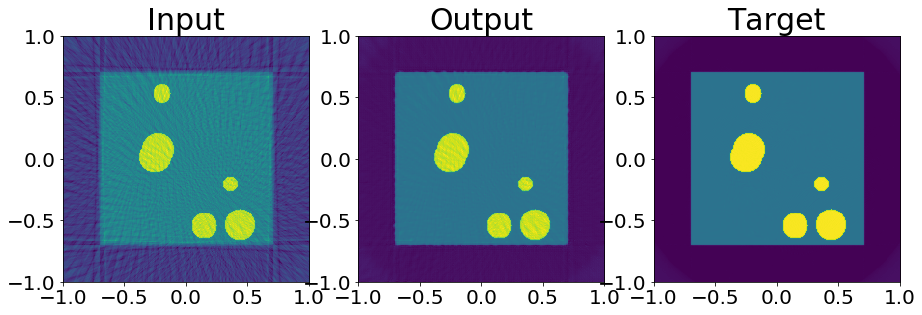
\includegraphics[width=\textwidth]{figures/sparse_angle_50_1} \
    \caption{Unseen test result from network trained on fifty projections}
\end{figure}

\begin{figure}[H]
\centering
     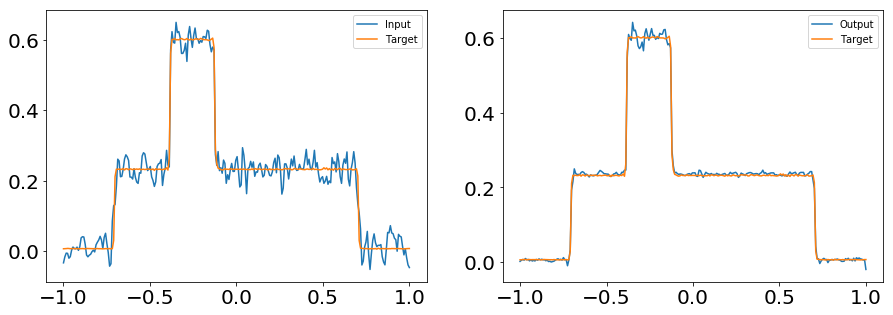
\includegraphics[width=\textwidth]{figures/sparse_angle_profile_50_1} \
    \caption{Profile through centre of output image and input image compared with target for network trained on fifty projections}
\end{figure}

Average Test loss : 2.12240107143

\begin{figure}[H]
\centering
     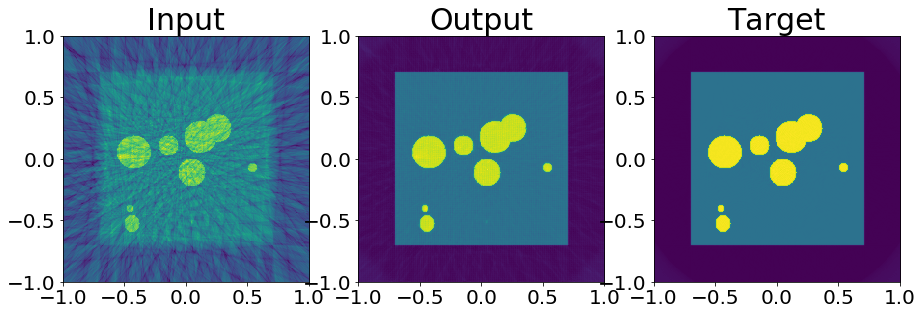
\includegraphics[width=\textwidth]{figures/sparse_angle_20_1} \
    \caption{Unseen test result from network trained on twenty projections}
\end{figure}

\begin{figure}[H]
\centering
     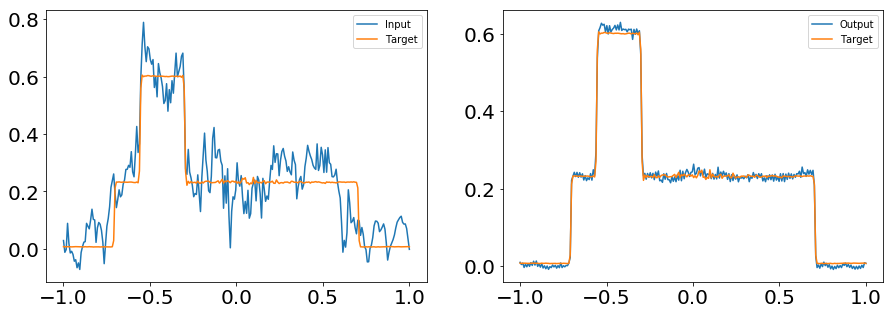
\includegraphics[width=\textwidth]{figures/sparse_angle_profile_20_1} \
    \caption{Profile through centre of output image and input image compared with target for network trained on twenty projections}
\end{figure}

Average Test loss : 2.34353055954

\begin{figure}[H]
\centering
     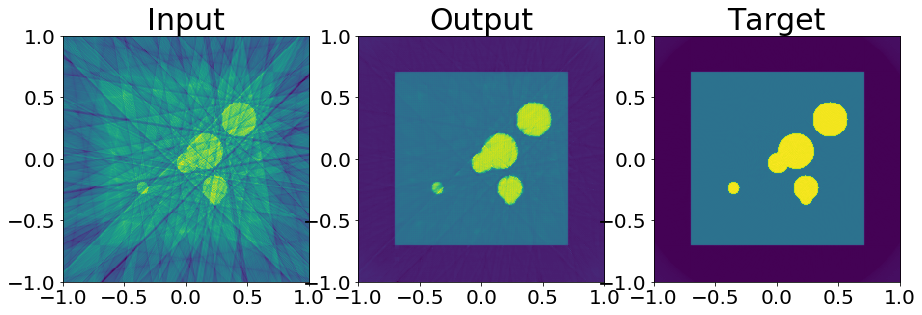
\includegraphics[width=\textwidth]{figures/sparse_angle_10_1} \
    \caption{Unseen test result from network trained on ten projections}
\end{figure}

\begin{figure}[H]
\centering
     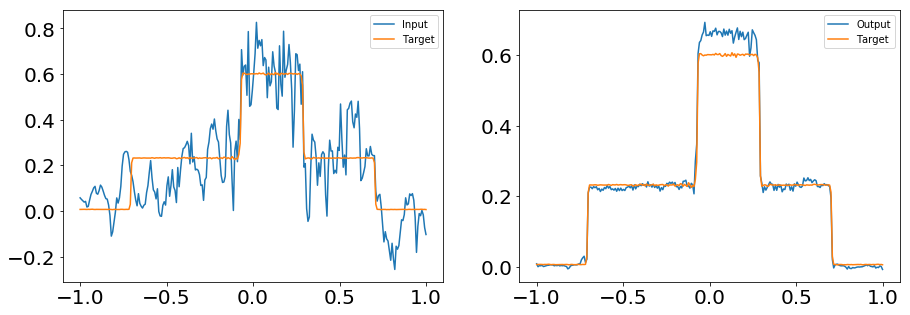
\includegraphics[width=\textwidth]{figures/sparse_angle_profile_10_1} \
    \caption{Profile through centre of output image and input image compared with target for network trained on ten projections}
\end{figure}

Average Test loss : 10.7825043774

\subsection{Sparse Angle reconstruction - Projection Domain}

\begin{figure}[H]
\centering
     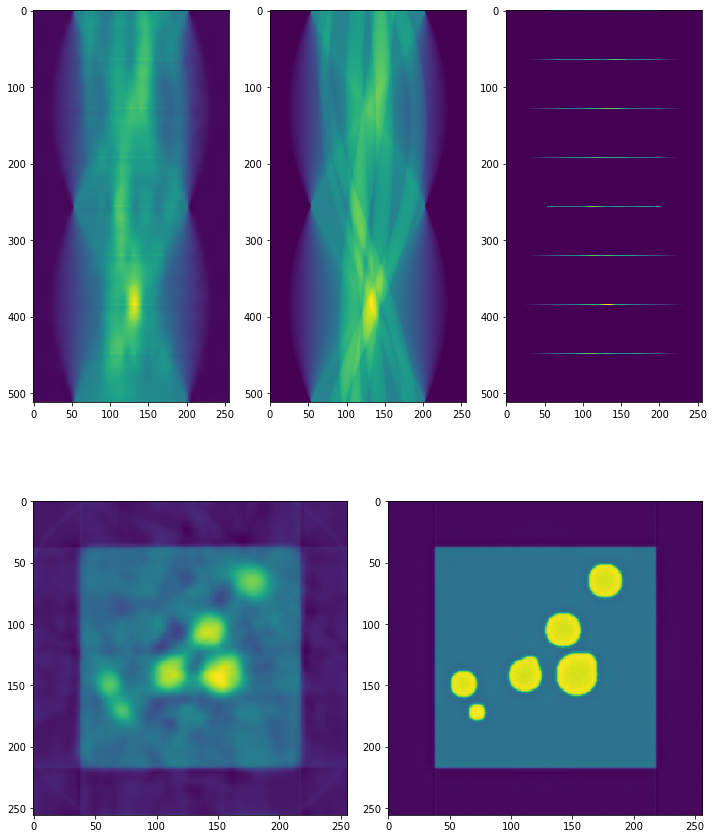
\includegraphics[width=\textwidth]{figures/sparse_sino_32_1} \
\end{figure}

\subsection{Polychromatic Artefact removal}

\begin{figure}[H]
\centering
     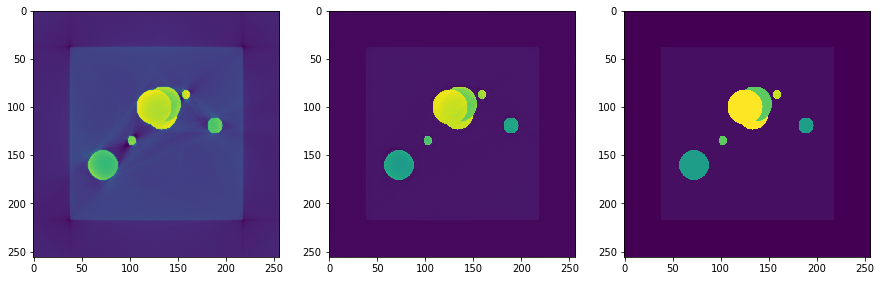
\includegraphics[width=\textwidth]{figures/poly_art_rem_ims_1} \
\end{figure}

\begin{figure}[H]
\centering
     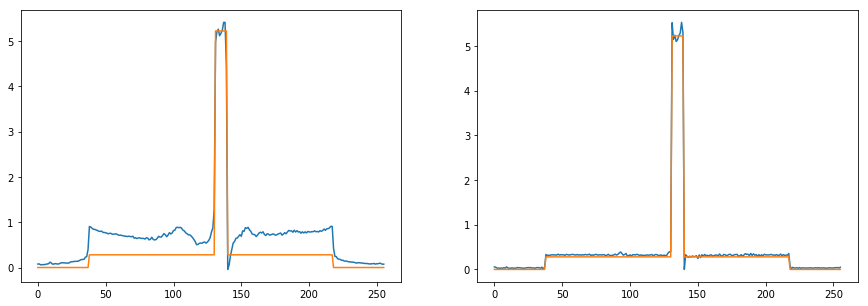
\includegraphics[width=\textwidth]{figures/poly_art_rem_profile_1} \
  \caption{This is   some figure side by side}
\end{figure}

Lorem ipsum dolor sit amet, consectetur adipiscing elit. Phasellus ut libero consequat, egestas ex sed, venenatis odio. Sed dictum cursus cursus. Cras dictum, metus in gravida maximus, ante risus tristique elit, at dignissim ipsum nibh a ex. Aliquam sit amet sodales eros. In lectus enim, feugiat eget massa nec, ultricies aliquam turpis. Nulla facilisi. Nulla commodo imperdiet erat, vitae interdum dolor bibendum a. Morbi feugiat ultrices libero id tincidunt. Vivamus luctus erat in fringilla pellentesque. Vivamus nec lorem tempor, mattis eros vel, egestas dui. Vestibulum scelerisque condimentum dolor. Proin convallis nulla dolor.

Donec eu tortor eget eros tincidunt fringilla. Curabitur fermentum vel magna sit amet consequat. Integer egestas lorem vel purus dictum facilisis. Duis sit amet urna ac neque gravida facilisis. Maecenas et erat ut eros laoreet fringilla. Quisque id turpis scelerisque, semper elit sit amet, consequat dolor. Vestibulum mauris turpis, viverra tempus justo vel, faucibus accumsan quam.

Nulla facilisi. Proin a ornare purus. Suspendisse sit amet sem malesuada, lobortis magna vitae, tincidunt leo. Sed in eros velit. Integer non odio nec arcu pharetra congue. Nulla eleifend tempor arcu. Proin odio nibh, dictum vitae diam sit amet, viverra rhoncus tortor. Nulla facilisi. Mauris id ligula quis ipsum accumsan eleifend. Sed vel neque lectus. Morbi vulputate tellus ut vestibulum bibendum. Etiam eu orci ut arcu porta scelerisque eu vitae turpis. Nullam orci nulla, venenatis quis tellus vel, vehicula bibendum metus.

Nulla placerat augue porttitor, condimentum tellus vel, pellentesque nulla. Ut sodales volutpat mauris. Phasellus facilisis arcu nisi, vitae aliquam augue finibus in. Donec quis bibendum arcu. Nunc viverra massa sed imperdiet tristique. Phasellus vel sollicitudin mi. Sed malesuada egestas sodales. Maecenas feugiat neque vitae vehicula laoreet. Vestibulum quis accumsan lorem. Suspendisse elementum mi a elit sagittis, vel rhoncus ex viverra. Orci varius natoque penatibus et magnis dis parturient montes, nascetur ridiculus mus. Cras lacinia, felis malesuada tristique luctus, sem odio iaculis massa, non molestie nulla est sit amet purus. Suspendisse id nisl ante. Donec lacus odio, vestibulum lobortis tristique id, venenatis vel dui.

Nullam vestibulum imperdiet pharetra. Integer venenatis posuere arcu a ultricies. Mauris vulputate elit ac arcu volutpat convallis. Fusce ultricies mauris ligula, vel mattis ex auctor nec. Fusce suscipit lacus id hendrerit condimentum. Praesent porttitor arcu quis tincidunt maximus. Nulla pulvinar mi enim, vel laoreet nunc blandit at. Maecenas volutpat nec magna eget pharetra. Aenean non nunc sagittis, rutrum lacus volutpat, pharetra dolor. Quisque diam lacus, condimentum sed dictum a, ornare in diam. Ut eu ante quis dui ullamcorper varius ut id diam. Aenean sit amet ornare tortor. Etiam mollis convallis odio. Mauris ut pulvinar odio.

Etiam malesuada eros risus, id volutpat mi imperdiet eu. Donec cursus lacus nunc, auctor tincidunt arcu fermentum nec. Donec est velit, eleifend eu fringilla ut, rhoncus et nisi. Aenean libero odio, congue at justo sit amet, volutpat suscipit turpis. Ut at finibus nulla. Fusce tincidunt eu mauris in suscipit. Sed suscipit ultricies risus in hendrerit. Donec et est interdum, tempus purus ac, lobortis elit. Fusce fringilla ex tempor diam tincidunt, cursus laoreet urna.

Lorem ipsum dolor sit amet, consectetur adipiscing elit. Phasellus ut libero consequat, egestas ex sed, venenatis odio. Sed dictum cursus cursus. Cras dictum, metus in gravida maximus, ante risus tristique elit, at dignissim ipsum nibh a ex. Aliquam sit amet sodales eros. In lectus enim, feugiat eget massa nec, ultricies aliquam turpis. Nulla facilisi. Nulla commodo imperdiet erat, vitae interdum dolor bibendum a. Morbi feugiat ultrices libero id tincidunt. Vivamus luctus erat in fringilla pellentesque. Vivamus nec lorem tempor, mattis eros vel, egestas dui. Vestibulum scelerisque condimentum dolor. Proin convallis nulla dolor.

Donec eu tortor eget eros tincidunt fringilla. Curabitur fermentum vel magna sit amet consequat. Integer egestas lorem vel purus dictum facilisis. Duis sit amet urna ac neque gravida facilisis. Maecenas et erat ut eros laoreet fringilla. Quisque id turpis scelerisque, semper elit sit amet, consequat dolor. Vestibulum mauris turpis, viverra tempus justo vel, faucibus accumsan quam.

Nulla facilisi. Proin a ornare purus. Suspendisse sit amet sem malesuada, lobortis magna vitae, tincidunt leo. Sed in eros velit. Integer non odio nec arcu pharetra congue. Nulla eleifend tempor arcu. Proin odio nibh, dictum vitae diam sit amet, viverra rhoncus tortor. Nulla facilisi. Mauris id ligula quis ipsum accumsan eleifend. Sed vel neque lectus. Morbi vulputate tellus ut vestibulum bibendum. Etiam eu orci ut arcu porta scelerisque eu vitae turpis. Nullam orci nulla, venenatis quis tellus vel, vehicula bibendum metus.

Nulla placerat augue porttitor, condimentum tellus vel, pellentesque nulla. Ut sodales volutpat mauris. Phasellus facilisis arcu nisi, vitae aliquam augue finibus in. Donec quis bibendum arcu. Nunc viverra massa sed imperdiet tristique. Phasellus vel sollicitudin mi. Sed malesuada egestas sodales. Maecenas feugiat neque vitae vehicula laoreet. Vestibulum quis accumsan lorem. Suspendisse elementum mi a elit sagittis, vel rhoncus ex viverra. Orci varius natoque penatibus et magnis dis parturient montes, nascetur ridiculus mus. Cras lacinia, felis malesuada tristique luctus, sem odio iaculis massa, non molestie nulla est sit amet purus. Suspendisse id nisl ante. Donec lacus odio, vestibulum lobortis tristique id, venenatis vel dui.

Nullam vestibulum imperdiet pharetra. Integer venenatis posuere arcu a ultricies. Mauris vulputate elit ac arcu volutpat convallis. Fusce ultricies mauris ligula, vel mattis ex auctor nec. Fusce suscipit lacus id hendrerit condimentum. Praesent porttitor arcu quis tincidunt maximus. Nulla pulvinar mi enim, vel laoreet nunc blandit at. Maecenas volutpat nec magna eget pharetra. Aenean non nunc sagittis, rutrum lacus volutpat, pharetra dolor. Quisque diam lacus, condimentum sed dictum a, ornare in diam. Ut eu ante quis dui ullamcorper varius ut id diam. Aenean sit amet ornare tortor. Etiam mollis convallis odio. Mauris ut pulvinar odio.

Etiam malesuada eros risus, id volutpat mi imperdiet eu. Donec cursus lacus nunc, auctor tincidunt arcu fermentum nec. Donec est velit, eleifend eu fringilla ut, rhoncus et nisi. Aenean libero odio, congue at justo sit amet, volutpat suscipit turpis. Ut at finibus nulla. Fusce tincidunt eu mauris in suscipit. Sed suscipit ultricies risus in hendrerit. Donec et est interdum, tempus purus ac, lobortis elit. Fusce fringilla ex tempor diam tincidunt, cursus laoreet urna.

\begin{figure}
    \centering
    \begin{subfigure}[t]{\linewidth}
        \centering
        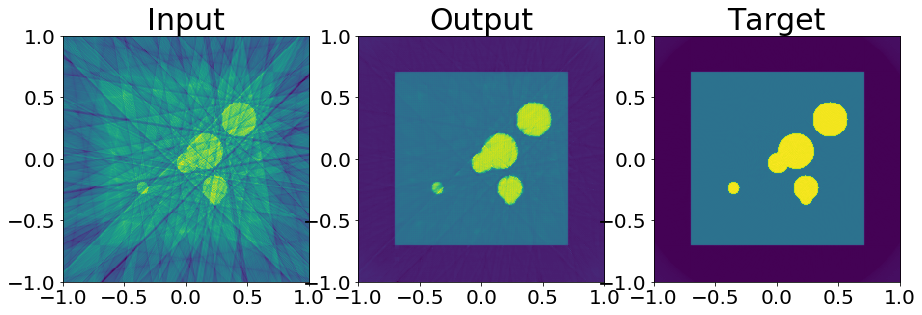
\includegraphics[width=\linewidth]{figures/sparse_angle_10_1} 
        \caption{Generic} \label{fig:timing1}
    \end{subfigure}
    \vspace{1cm}
    \begin{subfigure}[t]{\textwidth}
    \centering
        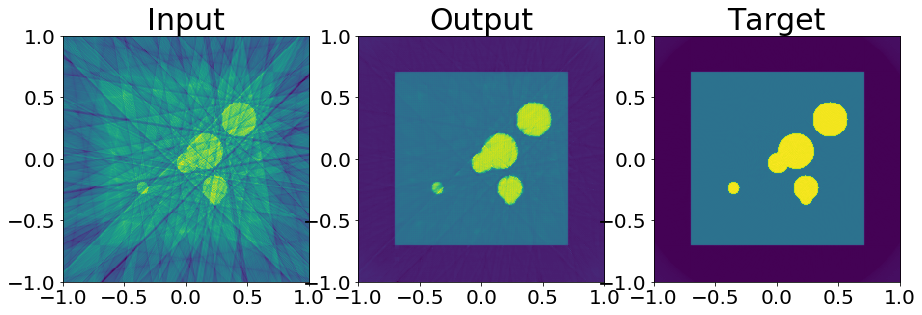
\includegraphics[width=\linewidth]{figures/sparse_angle_10_1} 
        \caption{Price regulation} \label{fig:timing3}
    \end{subfigure}
    \caption{Some general caption of all the figures. In (\subref{fig:timing1}) you can see a  green square....}
\end{figure}


\section{Discussion}

Lorem ipsum dolor sit amet, consectetur adipiscing elit. Phasellus ut libero consequat, egestas ex sed, venenatis odio. Sed dictum cursus cursus. Cras dictum, metus in gravida maximus, ante risus tristique elit, at dignissim ipsum nibh a ex. Aliquam sit amet sodales eros. In lectus enim, feugiat eget massa nec, ultricies aliquam turpis. Nulla facilisi. Nulla commodo imperdiet erat, vitae interdum dolor bibendum a. Morbi feugiat ultrices libero id tincidunt. Vivamus luctus erat in fringilla pellentesque. Vivamus nec lorem tempor, mattis eros vel, egestas dui. Vestibulum scelerisque condimentum dolor. Proin convallis nulla dolor.

Donec eu tortor eget eros tincidunt fringilla. Curabitur fermentum vel magna sit amet consequat. Integer egestas lorem vel purus dictum facilisis. Duis sit amet urna ac neque gravida facilisis. Maecenas et erat ut eros laoreet fringilla. Quisque id turpis scelerisque, semper elit sit amet, consequat dolor. Vestibulum mauris turpis, viverra tempus justo vel, faucibus accumsan quam.

Nulla facilisi. Proin a ornare purus. Suspendisse sit amet sem malesuada, lobortis magna vitae, tincidunt leo. Sed in eros velit. Integer non odio nec arcu pharetra congue. Nulla eleifend tempor arcu. Proin odio nibh, dictum vitae diam sit amet, viverra rhoncus tortor. Nulla facilisi. Mauris id ligula quis ipsum accumsan eleifend. Sed vel neque lectus. Morbi vulputate tellus ut vestibulum bibendum. Etiam eu orci ut arcu porta scelerisque eu vitae turpis. Nullam orci nulla, venenatis quis tellus vel, vehicula bibendum metus.

Nulla placerat augue porttitor, condimentum tellus vel, pellentesque nulla. Ut sodales volutpat mauris. Phasellus facilisis arcu nisi, vitae aliquam augue finibus in. Donec quis bibendum arcu. Nunc viverra massa sed imperdiet tristique. Phasellus vel sollicitudin mi. Sed malesuada egestas sodales. Maecenas feugiat neque vitae vehicula laoreet. Vestibulum quis accumsan lorem. Suspendisse elementum mi a elit sagittis, vel rhoncus ex viverra. Orci varius natoque penatibus et magnis dis parturient montes, nascetur ridiculus mus. Cras lacinia, felis malesuada tristique luctus, sem odio iaculis massa, non molestie nulla est sit amet purus. Suspendisse id nisl ante. Donec lacus odio, vestibulum lobortis tristique id, venenatis vel dui.

Nullam vestibulum imperdiet pharetra. Integer venenatis posuere arcu a ultricies. Mauris vulputate elit ac arcu volutpat convallis. Fusce ultricies mauris ligula, vel mattis ex auctor nec. Fusce suscipit lacus id hendrerit condimentum. Praesent porttitor arcu quis tincidunt maximus. Nulla pulvinar mi enim, vel laoreet nunc blandit at. Maecenas volutpat nec magna eget pharetra. Aenean non nunc sagittis, rutrum lacus volutpat, pharetra dolor. Quisque diam lacus, condimentum sed dictum a, ornare in diam. Ut eu ante quis dui ullamcorper varius ut id diam. Aenean sit amet ornare tortor. Etiam mollis convallis odio. Mauris ut pulvinar odio.

Etiam malesuada eros risus, id volutpat mi imperdiet eu. Donec cursus lacus nunc, auctor tincidunt arcu fermentum nec. Donec est velit, eleifend eu fringilla ut, rhoncus et nisi. Aenean libero odio, congue at justo sit amet, volutpat suscipit turpis. Ut at finibus nulla. Fusce tincidunt eu mauris in suscipit. Sed suscipit ultricies risus in hendrerit. Donec et est interdum, tempus purus ac, lobortis elit. Fusce fringilla ex tempor diam tincidunt, cursus laoreet urna.

Lorem ipsum dolor sit amet, consectetur adipiscing elit. Phasellus ut libero consequat, egestas ex sed, venenatis odio. Sed dictum cursus cursus. Cras dictum, metus in gravida maximus, ante risus tristique elit, at dignissim ipsum nibh a ex. Aliquam sit amet sodales eros. In lectus enim, feugiat eget massa nec, ultricies aliquam turpis. Nulla facilisi. Nulla commodo imperdiet erat, vitae interdum dolor bibendum a. Morbi feugiat ultrices libero id tincidunt. Vivamus luctus erat in fringilla pellentesque. Vivamus nec lorem tempor, mattis eros vel, egestas dui. Vestibulum scelerisque condimentum dolor. Proin convallis nulla dolor.

Donec eu tortor eget eros tincidunt fringilla. Curabitur fermentum vel magna sit amet consequat. Integer egestas lorem vel purus dictum facilisis. Duis sit amet urna ac neque gravida facilisis. Maecenas et erat ut eros laoreet fringilla. Quisque id turpis scelerisque, semper elit sit amet, consequat dolor. Vestibulum mauris turpis, viverra tempus justo vel, faucibus accumsan quam.

Nulla facilisi. Proin a ornare purus. Suspendisse sit amet sem malesuada, lobortis magna vitae, tincidunt leo. Sed in eros velit. Integer non odio nec arcu pharetra congue. Nulla eleifend tempor arcu. Proin odio nibh, dictum vitae diam sit amet, viverra rhoncus tortor. Nulla facilisi. Mauris id ligula quis ipsum accumsan eleifend. Sed vel neque lectus. Morbi vulputate tellus ut vestibulum bibendum. Etiam eu orci ut arcu porta scelerisque eu vitae turpis. Nullam orci nulla, venenatis quis tellus vel, vehicula bibendum metus.

Nulla placerat augue porttitor, condimentum tellus vel, pellentesque nulla. Ut sodales volutpat mauris. Phasellus facilisis arcu nisi, vitae aliquam augue finibus in. Donec quis bibendum arcu. Nunc viverra massa sed imperdiet tristique. Phasellus vel sollicitudin mi. Sed malesuada egestas sodales. Maecenas feugiat neque vitae vehicula laoreet. Vestibulum quis accumsan lorem. Suspendisse elementum mi a elit sagittis, vel rhoncus ex viverra. Orci varius natoque penatibus et magnis dis parturient montes, nascetur ridiculus mus. Cras lacinia, felis malesuada tristique luctus, sem odio iaculis massa, non molestie nulla est sit amet purus. Suspendisse id nisl ante. Donec lacus odio, vestibulum lobortis tristique id, venenatis vel dui.

Nullam vestibulum imperdiet pharetra. Integer venenatis posuere arcu a ultricies. Mauris vulputate elit ac arcu volutpat convallis. Fusce ultricies mauris ligula, vel mattis ex auctor nec. Fusce suscipit lacus id hendrerit condimentum. Praesent porttitor arcu quis tincidunt maximus. Nulla pulvinar mi enim, vel laoreet nunc blandit at. Maecenas volutpat nec magna eget pharetra. Aenean non nunc sagittis, rutrum lacus volutpat, pharetra dolor. Quisque diam lacus, condimentum sed dictum a, ornare in diam. Ut eu ante quis dui ullamcorper varius ut id diam. Aenean sit amet ornare tortor. Etiam mollis convallis odio. Mauris ut pulvinar odio.

Etiam malesuada eros risus, id volutpat mi imperdiet eu. Donec cursus lacus nunc, auctor tincidunt arcu fermentum nec. Donec est velit, eleifend eu fringilla ut, rhoncus et nisi. Aenean libero odio, congue at justo sit amet, volutpat suscipit turpis. Ut at finibus nulla. Fusce tincidunt eu mauris in suscipit. Sed suscipit ultricies risus in hendrerit. Donec et est interdum, tempus purus ac, lobortis elit. Fusce fringilla ex tempor diam tincidunt, cursus laoreet urna.

Lorem ipsum dolor sit amet, consectetur adipiscing elit. Phasellus ut libero consequat, egestas ex sed, venenatis odio. Sed dictum cursus cursus. Cras dictum, metus in gravida maximus, ante risus tristique elit, at dignissim ipsum nibh a ex. Aliquam sit amet sodales eros. In lectus enim, feugiat eget massa nec, ultricies aliquam turpis. Nulla facilisi. Nulla commodo imperdiet erat, vitae interdum dolor bibendum a. Morbi feugiat ultrices libero id tincidunt. Vivamus luctus erat in fringilla pellentesque. Vivamus nec lorem tempor, mattis eros vel, egestas dui. Vestibulum scelerisque condimentum dolor. Proin convallis nulla dolor.

Donec eu tortor eget eros tincidunt fringilla. Curabitur fermentum vel magna sit amet consequat. Integer egestas lorem vel purus dictum facilisis. Duis sit amet urna ac neque gravida facilisis. Maecenas et erat ut eros laoreet fringilla. Quisque id turpis scelerisque, semper elit sit amet, consequat dolor. Vestibulum mauris turpis, viverra tempus justo vel, faucibus accumsan quam.

Nulla facilisi. Proin a ornare purus. Suspendisse sit amet sem malesuada, lobortis magna vitae, tincidunt leo. Sed in eros velit. Integer non odio nec arcu pharetra congue. Nulla eleifend tempor arcu. Proin odio nibh, dictum vitae diam sit amet, viverra rhoncus tortor. Nulla facilisi. Mauris id ligula quis ipsum accumsan eleifend. Sed vel neque lectus. Morbi vulputate tellus ut vestibulum bibendum. Etiam eu orci ut arcu porta scelerisque eu vitae turpis. Nullam orci nulla, venenatis quis tellus vel, vehicula bibendum metus.

Nulla placerat augue porttitor, condimentum tellus vel, pellentesque nulla. Ut sodales volutpat mauris. Phasellus facilisis arcu nisi, vitae aliquam augue finibus in. Donec quis bibendum arcu. Nunc viverra massa sed imperdiet tristique. Phasellus vel sollicitudin mi. Sed malesuada egestas sodales. Maecenas feugiat neque vitae vehicula laoreet. Vestibulum quis accumsan lorem. Suspendisse elementum mi a elit sagittis, vel rhoncus ex viverra. Orci varius natoque penatibus et magnis dis parturient montes, nascetur ridiculus mus. Cras lacinia, felis malesuada tristique luctus, sem odio iaculis massa, non molestie nulla est sit amet purus. Suspendisse id nisl ante. Donec lacus odio, vestibulum lobortis tristique id, venenatis vel dui.

Nullam vestibulum imperdiet pharetra. Integer venenatis posuere arcu a ultricies. Mauris vulputate elit ac arcu volutpat convallis. Fusce ultricies mauris ligula, vel mattis ex auctor nec. Fusce suscipit lacus id hendrerit condimentum. Praesent porttitor arcu quis tincidunt maximus. Nulla pulvinar mi enim, vel laoreet nunc blandit at. Maecenas volutpat nec magna eget pharetra. Aenean non nunc sagittis, rutrum lacus volutpat, pharetra dolor. Quisque diam lacus, condimentum sed dictum a, ornare in diam. Ut eu ante quis dui ullamcorper varius ut id diam. Aenean sit amet ornare tortor. Etiam mollis convallis odio. Mauris ut pulvinar odio.

Etiam malesuada eros risus, id volutpat mi imperdiet eu. Donec cursus lacus nunc, auctor tincidunt arcu fermentum nec. Donec est velit, eleifend eu fringilla ut, rhoncus et nisi. Aenean libero odio, congue at justo sit amet, volutpat suscipit turpis. Ut at finibus nulla. Fusce tincidunt eu mauris in suscipit. Sed suscipit ultricies risus in hendrerit. Donec et est interdum, tempus purus ac, lobortis elit. Fusce fringilla ex tempor diam tincidunt, cursus laoreet urna.

\chapter{Conclusion}

orem ipsum dolor sit amet, consectetur adipiscing elit. Vivamus at pulvinar nisi. Phasellus hendrerit, diam placerat interdum iaculis, mauris justo cursus risus, in viverra purus eros at ligula. Ut metus justo, consequat a tristique posuere, laoreet nec nibh. Etiam et scelerisque mauris. Phasellus vel massa magna. Ut non neque id tortor pharetra bibendum vitae sit amet nisi. Duis nec quam quam, sed euismod justo. Pellentesque eu tellus vitae ante tempus malesuada. Nunc accumsan, quam in congue consequat, lectus lectus dapibus erat, id aliquet urna neque at massa. Nulla facilisi. Morbi ullamcorper eleifend posuere. Donec libero leo, faucibus nec bibendum at, mattis et urna. Proin consectetur, nunc ut imperdiet lobortis, magna neque tincidunt lectus, id iaculis nisi justo id nibh. Pellentesque vel sem in erat vulputate faucibus molestie ut lorem.

Quisque tristique urna in lorem laoreet at laoreet quam congue. Donec dolor turpis, blandit non imperdiet aliquet, blandit et felis. In lorem nisi, pretium sit amet vestibulum sed, tempus et sem. Proin non ante turpis. Nulla imperdiet fringilla convallis. Vivamus vel bibendum nisl. Pellentesque justo lectus, molestie vel luctus sed, lobortis in libero. Nulla facilisi. Aliquam erat volutpat. Suspendisse vitae nunc nunc. Sed aliquet est suscipit sapien rhoncus non adipiscing nibh consequat. Aliquam metus urna, faucibus eu vulputate non, luctus eu justo. 

%% ----------------------------------------------------------------
% Now begin the Appendices, including them as separate files

\addtocontents{toc}{\vspace{2em}} % Add a gap in the Contents, for aesthetics

\appendix % Cue to tell LaTeX that the following 'chapters' are Appendices

% \chapter{An Appendix}

Lorem ipsum dolor sit amet, consectetur adipiscing elit. Vivamus at pulvinar nisi. Phasellus hendrerit, diam placerat interdum iaculis, mauris justo cursus risus, in viverra purus eros at ligula. Ut metus justo, consequat a tristique posuere, laoreet nec nibh. Etiam et scelerisque mauris. Phasellus vel massa magna. Ut non neque id tortor pharetra bibendum vitae sit amet nisi. Duis nec quam quam, sed euismod justo. Pellentesque eu tellus vitae ante tempus malesuada. Nunc accumsan, quam in congue consequat, lectus lectus dapibus erat, id aliquet urna neque at massa. Nulla facilisi. Morbi ullamcorper eleifend posuere. Donec libero leo, faucibus nec bibendum at, mattis et urna. Proin consectetur, nunc ut imperdiet lobortis, magna neque tincidunt lectus, id iaculis nisi justo id nibh. Pellentesque vel sem in erat vulputate faucibus molestie ut lorem.

Quisque tristique urna in lorem laoreet at laoreet quam congue. Donec dolor turpis, blandit non imperdiet aliquet, blandit et felis. In lorem nisi, pretium sit amet vestibulum sed, tempus et sem. Proin non ante turpis. Nulla imperdiet fringilla convallis. Vivamus vel bibendum nisl. Pellentesque justo lectus, molestie vel luctus sed, lobortis in libero. Nulla facilisi. Aliquam erat volutpat. Suspendisse vitae nunc nunc. Sed aliquet est suscipit sapien rhoncus non adipiscing nibh consequat. Aliquam metus urna, faucibus eu vulputate non, luctus eu justo.

Donec urna leo, vulputate vitae porta eu, vehicula blandit libero. Phasellus eget massa et leo condimentum mollis. Nullam molestie, justo at pellentesque vulputate, sapien velit ornare diam, nec gravida lacus augue non diam. Integer mattis lacus id libero ultrices sit amet mollis neque molestie. Integer ut leo eget mi volutpat congue. Vivamus sodales, turpis id venenatis placerat, tellus purus adipiscing magna, eu aliquam nibh dolor id nibh. Pellentesque habitant morbi tristique senectus et netus et malesuada fames ac turpis egestas. Sed cursus convallis quam nec vehicula. Sed vulputate neque eget odio fringilla ac sodales urna feugiat.

Phasellus nisi quam, volutpat non ullamcorper eget, congue fringilla leo. Cras et erat et nibh placerat commodo id ornare est. Nulla facilisi. Aenean pulvinar scelerisque eros eget interdum. Nunc pulvinar magna ut felis varius in hendrerit dolor accumsan. Nunc pellentesque magna quis magna bibendum non laoreet erat tincidunt. Nulla facilisi.

Duis eget massa sem, gravida interdum ipsum. Nulla nunc nisl, hendrerit sit amet commodo vel, varius id tellus. Lorem ipsum dolor sit amet, consectetur adipiscing elit. Nunc ac dolor est. Suspendisse ultrices tincidunt metus eget accumsan. Nullam facilisis, justo vitae convallis sollicitudin, eros augue malesuada metus, nec sagittis diam nibh ut sapien. Duis blandit lectus vitae lorem aliquam nec euismod nisi volutpat. Vestibulum ornare dictum tortor, at faucibus justo tempor non. Nulla facilisi. Cras non massa nunc, eget euismod purus. Nunc metus ipsum, euismod a consectetur vel, hendrerit nec nunc.	% Appendix Title

%\input{Appendices/AppendixB} % Appendix Title

%\input{Appendices/AppendixC} % Appendix Title

\addtocontents{toc}{\vspace{2em}}  % Add a gap in the Contents, for aesthetics
\backmatter

%% ----------------------------------------------------------------
\label{Bibliography}
\lhead{\emph{Bibliography}}  % Change the left side page header to "Bibliography"
\bibliographystyle{unsrtnat}  % Use the "unsrtnat" BibTeX style for formatting the Bibliography
\bibliography{Bibliography}  % The references (bibliography) information are stored in the file named "Bibliography.bib"

\end{document}  % The End
%% ----------------------------------------------------------------
